\artigotrue
\chapter{THE SANTA MARIA DATASET. PART I -- SOIL DATA}
\chapternote{Collaborated in the preparation of this chapter: Pablo Miguel (UFPel), Jean Michel Moura Bueno 
(UFSM), Ricardo Simão Diniz Dalmolin (UFSM), Andrisa Balbinot (UFSM), Lúcia Helena Cunha dos Anjos (UFRRJ), 
Gustavo de Mattos Vasques (Embrapa Solos), Gerard B. M. Heuvelink (ISRIC -- World Soil Information), and Ad 
van Oostrum (ISRIC -- World Soil Information).}
\shorttitle{Soil Data}
\label{chap:chap04}
%\SweaveUTF8


\def\ptkeys{Modelagem espacial do solo. Amostragem intencional. Dados legados. Descrição do solo no campo. 
Análise laboratorial do solo}
\begin{chapterabstract}{brazilian}{\ptkeys}
O \emph{conjunto de dados de Santa Maria} compreende dados do solo de $n = 410$  observações feitas entre 
2008 e 2013 na bacia do reservatório do Departamento Nacional de Obras de Saneamento-Companhia Riograndense de 
Saneamento (DNOS-CORSAN), localizada no estado brasileiro do Rio Grande do Sul. Esses dados do solo foram 
produzidos no âmbito de projetos de pesquisa que visam a produção de mapas semi-detalhados do solo e do
uso da terra, e prever o estoque superficial de carbono no solo e sua vulnerabilidade à erosão. Todos os 
locais de observação foram selecionados intencionalmente ou por conveniência. Várias características 
ambientais foram descritas nos locais de observação, tais como o uso da terra, geologia, classificação do 
solo, declividade, condições de drenagem, presença de fragmentos grosseiros e afloramentos rochosos, cobertura 
do solo com vegetação, entre outras peculiaridades de cada local de observação que não foram registradas de 
uma forma sistemática. As amostras do solo foram submetidos à análise de laboratório para determinar o 
conteúdo de carbono orgânico no solo, a distribuição do tamanho de partículas, a densidade e o conteúdo de 
bases (cálcio, magnésio, potássio e sódio) e acidez trocáveis. A capacidade de troca de cátions efetiva foi 
calculada como a soma das bases e acidez trocáveis. Os dados do solo estão disponíveis gratuitamente em um 
repositório hospedado no GitHub. Eles incluem a identificação de todos os locais de observação, as suas 
coordenadas geográficas, e dados de campo e de laboratório. O número de repetições de laboratório e o desvio 
padrão amostral também são fornecidos.

\end{chapterabstract}

\def\enkeys{Spatial soil modelling. Purposive sampling. Legacy data. Soil field description. Soil laboratory 
analysis}
  
\begin{chapterabstract}{english}{\enkeys}
The \emph{Santa Maria dataset} comprises soil data from $n = 410$ soil observations made between \num{2008} 
and \num{2013} in the catchment of the reservoir of the \textit{Departamento Nacional de Obras de 
Saneamento}-\textit{Companhia Riograndense de Saneamento} (DNOS-CORSAN), located in the southern Brazilian 
state of Rio Grande do Sul. These soil data were produced within the scope of research projects that aimed at 
producing semi-detailed soil and land use maps, and predicting topsoil carbon stock and vulnerability to 
erosion. All observation locations were selected purposively or by convenience. Several environmental 
features were described at the observation locations, such as land use, geology, soil classification, slope, 
drainage condition, presence of coarse fragments and rock outcrops, soil coverage with vegetation, among 
other peculiarities of each observation location that were not recorded in a systematic way. Soil samples were 
submitted to laboratory analysis to determine the soil organic carbon content, particle size distribution, 
bulk density, and the content of exchangeable bases (calcium, magnesium, potassium, and sodium) and acidity. 
The effective cation exchange capacity was calculated as the sum of exchangeable bases and acidity. The soil 
data is freely available in a repository hosted in GitHub. These include the identification of all observation 
locations, their geographic coordinates, and field and laboratory data. The number of laboratory replicates 
and the sample standard deviation is provided as well.
\end{chapterabstract}

\formatchapter

\section{INTRODUCTION}
\label{sec:chap04-introduction}

The \emph{Santa Maria dataset} comprises soil data from $n = 410$ soil observations made between \num{2004} 
and \num{2013} in the catchment of the reservoir of the \textit{Departamento Nacional de Obras de 
Saneamento}-\textit{Companhia Riograndense de Saneamento} (DNOS-CORSAN), henceforth called \emph{DNOS 
catchment}, located in the southern border of the Plateau of the Paraná Sedimentary Basin, in the city of 
Santa Maria, state of Rio Grande do Sul, Brazil. Soil observations cover the northern sector of the DNOS 
catchment -- an area of \SI{\pm2000}{\hectare}, which corresponds to \SI{\pm60}{\percent} of the entire 
catchment. These soil data were produced during the development of research projects that aimed at producing 
semi-detailed soil and land use maps (\scale{25000}) \cite{Pedron2005, Miguel2010, SamuelRosaEtAl2011a, 
MiguelEtAl2012}, and predicting topsoil carbon stock and vulnerability to erosion \cite{Samuel-Rosa2009, 
MouraBueno2012, Miguel2013}.

% Footnote %%%%%
\def\foottropics{\footnote{The reader should be aware that soil science evolved in Brazil following a somewhat 
different pathway than in the countries of the northern hemisphere due to the specific soil features of 
tropical and subtropical regions. Methods have been adapted along the years, possibly leading to nomenclature 
mismatches. The reader is invited to contribute to solve any problems in this document.}}

This chapter presents a thorough description of the soil data contained in the Santa Maria dataset. A 
thorough description of the procedures for soil sampling and description, as well as the analytical methods 
employed\foottropics{} is given. Soil data is also described using summary plots with descriptive statistics.

The chapter is divided in four sections. \autoref{sec:chap04-database} presents general information about 
the data, as well as the structure of the database where they have been stored and managed. Next, 
\autoref{sec:chap04-sampling} describes how field soil observation was carried out in each of the different 
project that contributed with soil data to the Santa Maria dataset. Methods used to describe the soil in the 
field are described in \autoref{sec:chap04-field-description}. \autoref{sec:chap04-laboratory} closes the 
chapter with a description of the laboratory methods used to produce data on physical and chemical soil 
properties.

\section{DATABASE STRUCTURE}
\label{sec:chap04-database}

The soil data contained in the Santa Maria dataset, as well as the code used in its processing, is freely 
available in the web-based \git{} repository \github{}. This is the same repository containing the ground 
control data (\autoref{sec:chap05-database}) The repository has the following folder structured:

\begin{verbatim}
dnos-sm-rs-general
|- code/                # source code folder
|  - R/                 # R source code folder
|    - general.R        # R source code file
|
|- data/                # soil data folder
|  - fieldData.csv      # field data file
|  - fieldMetadata.csv  # field metadata file
|  - labData.csv        # laboratory data file
|  - labMetadata.csv    # laboratory metadata file
|- README.md            # description of the repository
\end{verbatim}

\def\wgs{\href{http://spatialreference.org/ref/epsg/4326/}{\texttt{EPSG:4326}}}

Soil data files are available as comma-separated values (CSV) files. The identification of all observation 
locations, their geographic coordinates, and field and laboratory data are contained in files 
\texttt{fieldData.csv} and \texttt{labData.csv}, respectively. Files \texttt{fieldMetadata.csv} and 
\texttt{labMetadata.csv} contain the metadata. The coordinate reference system (CRS) is \texttt{WGS 84}, coded 
\wgs{} by the European Petroleum Survey Group (\href{http://www.epsg.org/}{EPSG}).

Every soil property is identified with a code composed of three or four capital letters. For example, soil 
organic carbon is identified with \texttt{ORCA}. A column containing the number of laboratory replicates is 
identified with the code of the soil property followed by the letter \q{N}. The column containing the sample 
standard deviation is identified in the same manner, but using \q{SD}. For example, \texttt{ORCA\_N} and 
\texttt{ORCA\_SD}.

\section{FIELD SAMPLING}
\label{sec:chap04-sampling}

The Santa Maria dataset is composed of three subsets which are described in the next three sections. Together, 
these subsets yield a sampling density of about \num{\pm0.18}~observations per hectare, with an average 
separation distance between two neighbouring points of \SI{180}{\metre}, minimum and maximum separation 
distances of \num{18} and \SI{328}{\metre}, \SI{95}{\percent} of neighbouring observations being separated by 
more than \SI{49}{\metre}.

\subsection{Subset I}

The first subset ($n = 340$, \autoref{fig:chap04-subsets-I-III}) was produced between 2008 and 20011 as part 
of projects that aimed at producing semi-detailed soil and land use maps, and predicting topsoil carbon stock 
and vulnerability to erosion \cite{Samuel-Rosa2009, SamuelRosaEtAl2011a, MiguelEtAl2012, Moura-BuenoEtAl2012, 
Samuel-RosaEtAl2013}. The researchers faced several difficulties with a budget cut and shortage of workforce. 
They also had restricted access to several areas due to geographic barriers and prohibition of access by some 
landowners. These difficulties forced the researchers to reduce the originally aimed number of observations 
($n = 500$) during the development of the project.

All observation locations were selected purposively or by convenience. Tacit knowledge 
(\autoref{sec:chap02-discrete} and \autoref{sec:chap07-elicited}) was the main tool to choose the observation 
locations, a process that was carried out in the office using \SI{1}{\metre} spatial resolution Google 
Earth\rr{} imagery of the years of \num{2008} and \num{2009}. The main goal of the researchers was to obtain a 
sample that they understood as being representative of the different landforms, land uses, and soil taxa 
present in the DNOS catchment. They also wanted the observations to be spread throughout the entire DNOS 
catchment.

% Footnote %%%%%
\def\footsupport{\footnote{\emph{Sample support} refers to the shape, size and orientation of sampling units, 
the latter being the smallest single entity that we are able or choose to observe in the universe of interest, 
i.e. the sampling region. A discrete universe such as a forest is defined by the collection of these single 
entities. However, by definition, such single entities have no real, physical existence in continuous 
universes such as the soil -- their \q{existence} require our prior, more or less arbitrary, definition of 
their shape, size and orientation. This definition is usually based on theoretical and practical 
considerations. For example, the sampling unit can be defined as a roughly polygonal block that is large 
enough to encompass the pattern of small-scale local vertical (\SI{\leq2}{\m}) and horizontal 
(1--\SI{10}{\square\metre}) variability of soil properties -- a pedon. Depending on the size of the sampling 
unit relative to the universe of interest, the sample support is referred to as \emph{areal} or \emph{point} 
sample support. A pedon of \SI{10}{\square\metre} area observed in an agricultural field of \SI{1}{\hectare} 
corresponds to the \emph{areal sample support}. However, the same pedon observed in a catchment of 
\SI{200}{\hectare} would correspond to the \emph{point sample support}.}}

At the observation locations, the researchers defined an area of \SI{\pm100}{\metre\squared} within which they 
opened three soil pits up to a depth of \SI{20}{\centi\metre}. Soil samples were collected up to a depth of 
\SI{20}{\centi\metre}, the depth being measured with a ruler. The resulting sampling depth of Subset I varies 
from \num{2} to \SI{20}{\centi\metre}, with an average of \SI{17}{\centi\metre}. This variation of the 
vertical sampling support\footsupport{} was not a problem for the researchers because their goal was to sample 
the \emph{topsoil}. The topsoil was defined as the topmost soil layer, with a thickness equal or inferior to 
\SI{20}{\centi\metre}, being the soil layer most susceptible to degradation induced by poor agricultural 
practices and land use changes.

Soil samples from the three pits opened in each sampling area were used to produce a composite sample which 
was used for laboratory analyses. Subsurface soil features were observed with an auger in each pit, and the 
average (continuous variables) or most common (categorical variables) value recorded. Note that soil sampling 
was done using an areal horizontal support -- an area of \SI{\pm100}{\metre\squared}. However, the shape and 
exact area of the sampling units are unknown, and georeferencing took place at point support.

\begin{figure}[!ht]
\centering
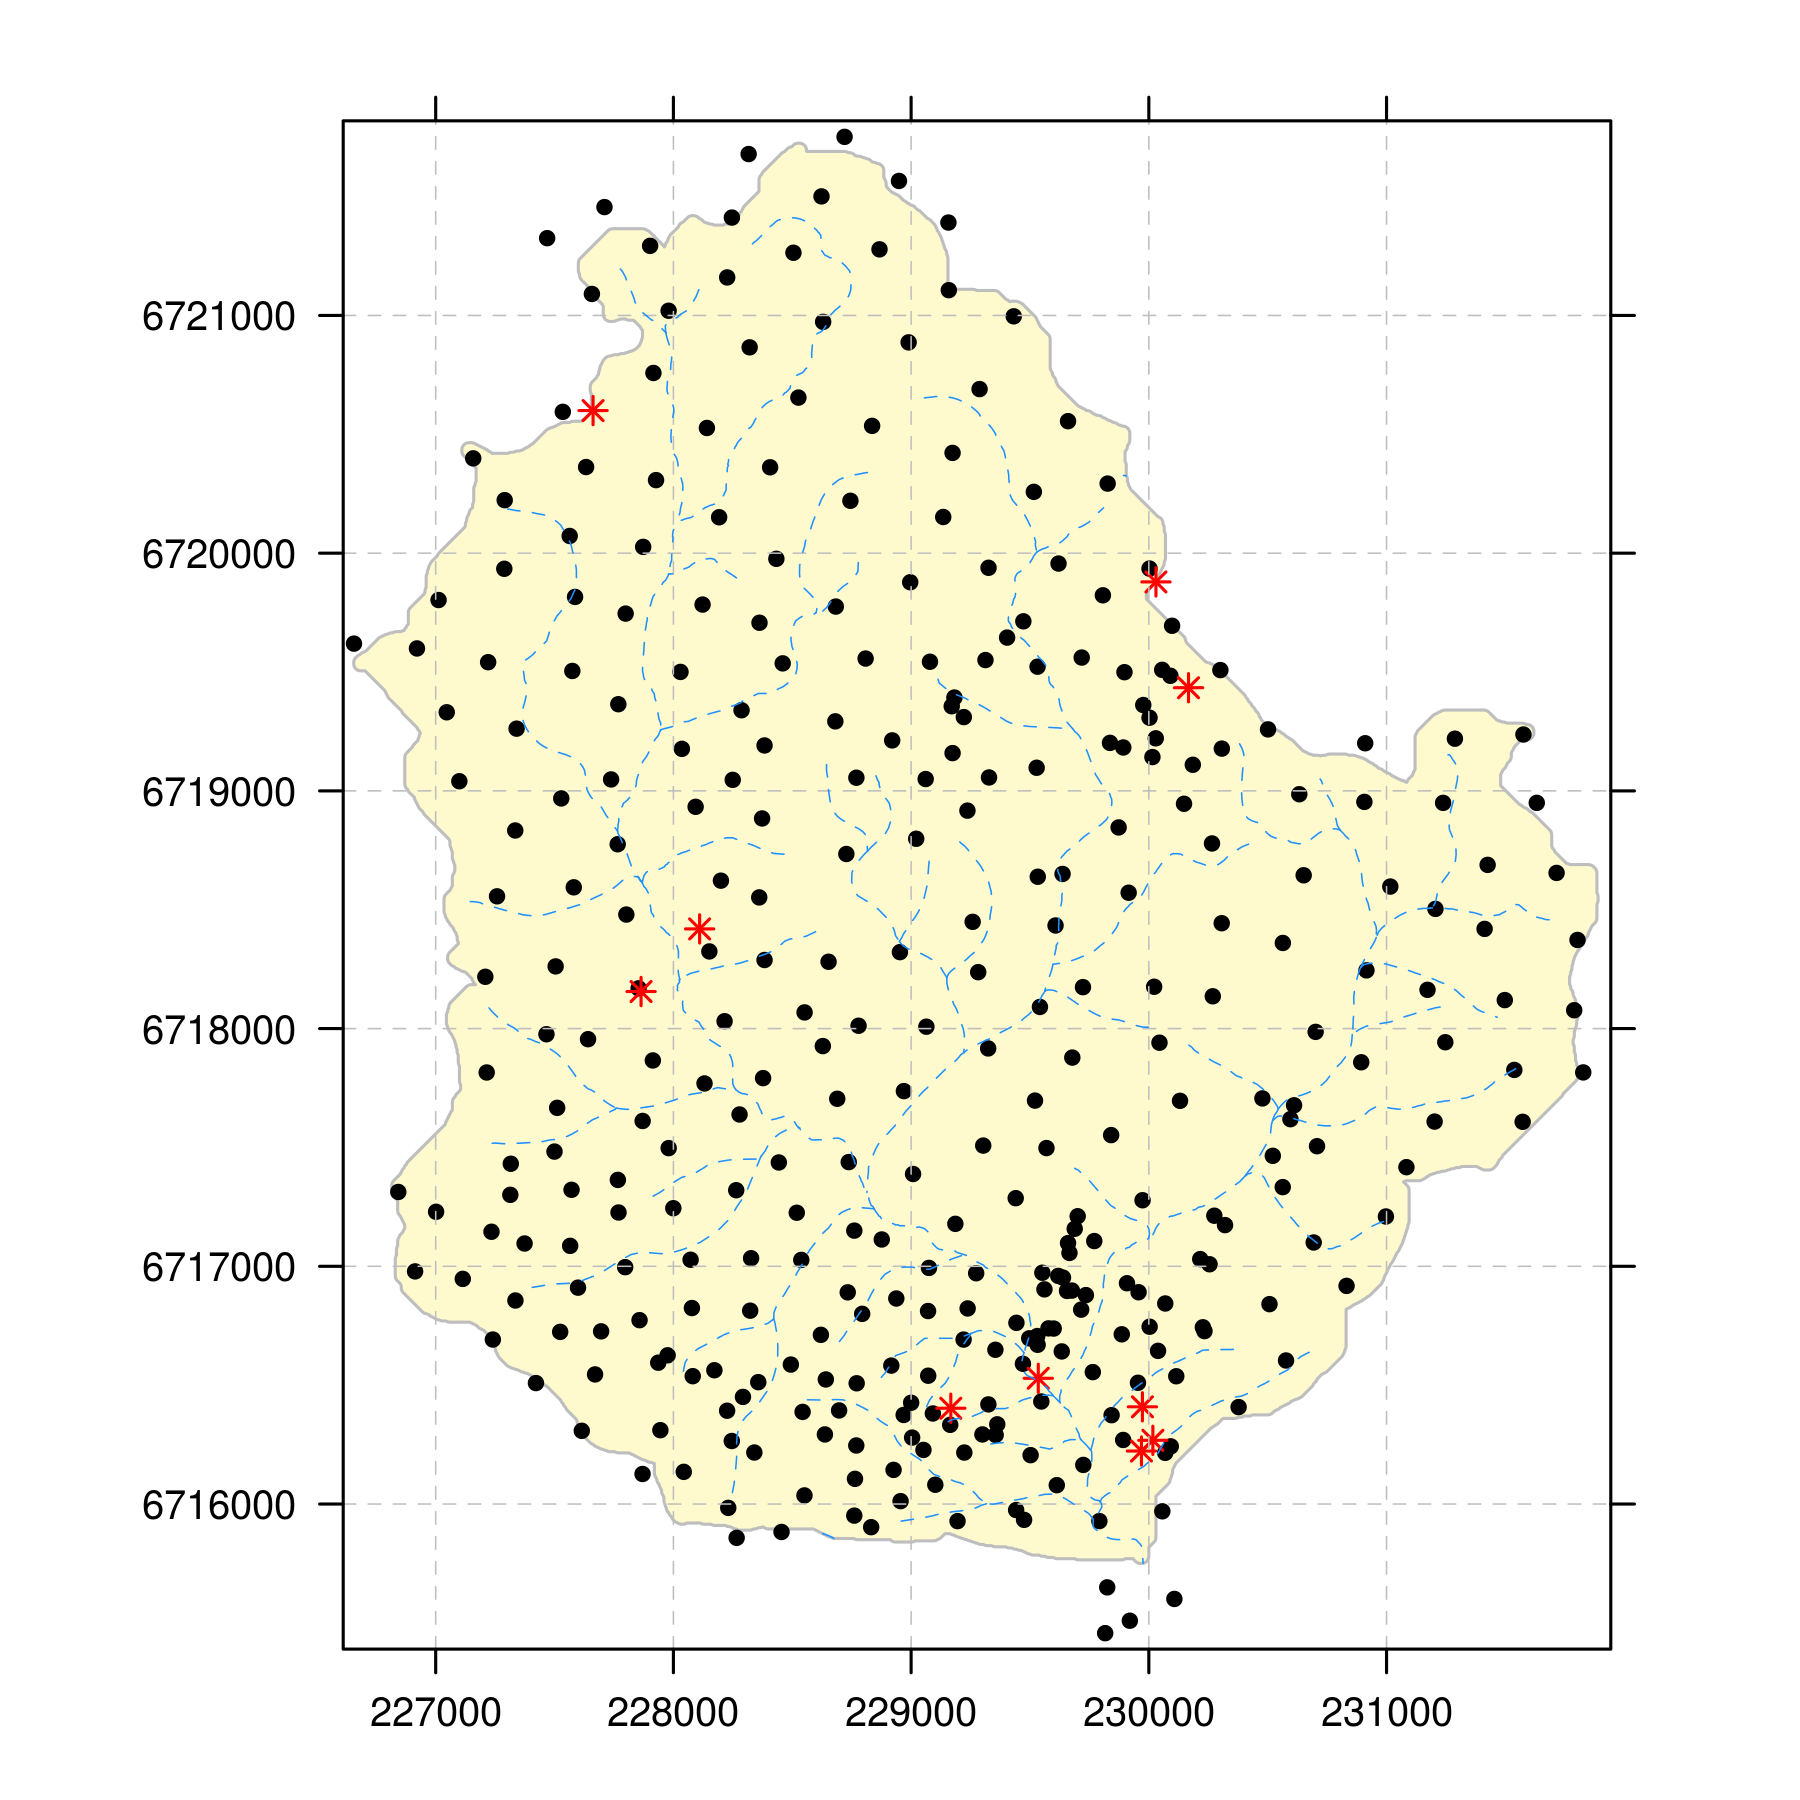
\includegraphics[width=0.90\textwidth]{fig/chap04-subsets-I-III}
\caption[Spatial distribution of \emph{Subset I} and \emph{Subset III}.]{Spatial distribution of the soil 
observations contained in \emph{Subset I} ($n = 340$, black solid circles) and \emph{Subset III} ($n = 
10$, red stars) of the Santa Maria dataset. The drainage network is shown in the background (blue 
dashed line) to give an idea of how the locations of soil observations is related to terrain features.}
\label{fig:chap04-subsets-I-III}
\end{figure}

Georeferencing was done in the field using a Global Navigation Satellite System (GNSS) receiver with a 
horizontal positional error of less than \SI{8}{\metre} positioned approximately at the centre of the
sampling area. Sometimes, the horizontal positional error was larger than \SI{8}{\metre} due the effects
of vegetation, terrain, and satellite configuration. In these cases, observation locations were georeferenced 
in the office using \SI{1}{\metre} spatial resolution Google Earth\rr{} imagery with positional horizontal 
error of \SI{6}{\metre} (\autoref{tab:chap05-google-geo-val}).

Every observation was identified with a number in increasing order, following the order in which the 
observations were made (\num{001}--\num{340}). A total of \num{17}~field campaigns were carried out, yielding 
an observation density of about \num{18}~observations per \si{\kilo\metre\squared} (\autoref{chap:chap07}).

\subsection{Subset II}
\label{sec:chap04-subset-ii}

The second subset ($n = 60$, \autoref{fig:chap04-subset-II}) was produced in the years \num{2012} and 
\num{2013}, and was intended to constitute an independent dataset for validation purposes. Because of the many 
access limitations (geographic barriers and prohibition by landowners) and shortage of workforce, budget, 
infrastructure and time faced in previous field campaigns, researchers chose to employ transect (cluster) 
sampling \cite{MiguelEtAl2012, Moura-BuenoEtAl2012, Samuel-RosaEtAl2013}. They started defining the population 
of transects using their knowledge of the study area, taking into account the factors that they thought 
determined the spatial distribution of soil properties. Each researcher (three) delineated $m = 60$ easily 
accessible, straight transects of \SI{400}{\metre} following the spatial gradients of selected environmental 
features (topography, geology, vegetation, land use, and soils), totalling 180 transects. Accordingly, 
knowledge of existing roads, human settlements, water bodies, and other access limitations was used as well. 
The activity was carried out using \SI{1}{\metre} spatial resolution Google Earth\rr{} imagery of the years of 
\num{2008} and \num{2009}.

\begin{figure}[!ht]
\centering
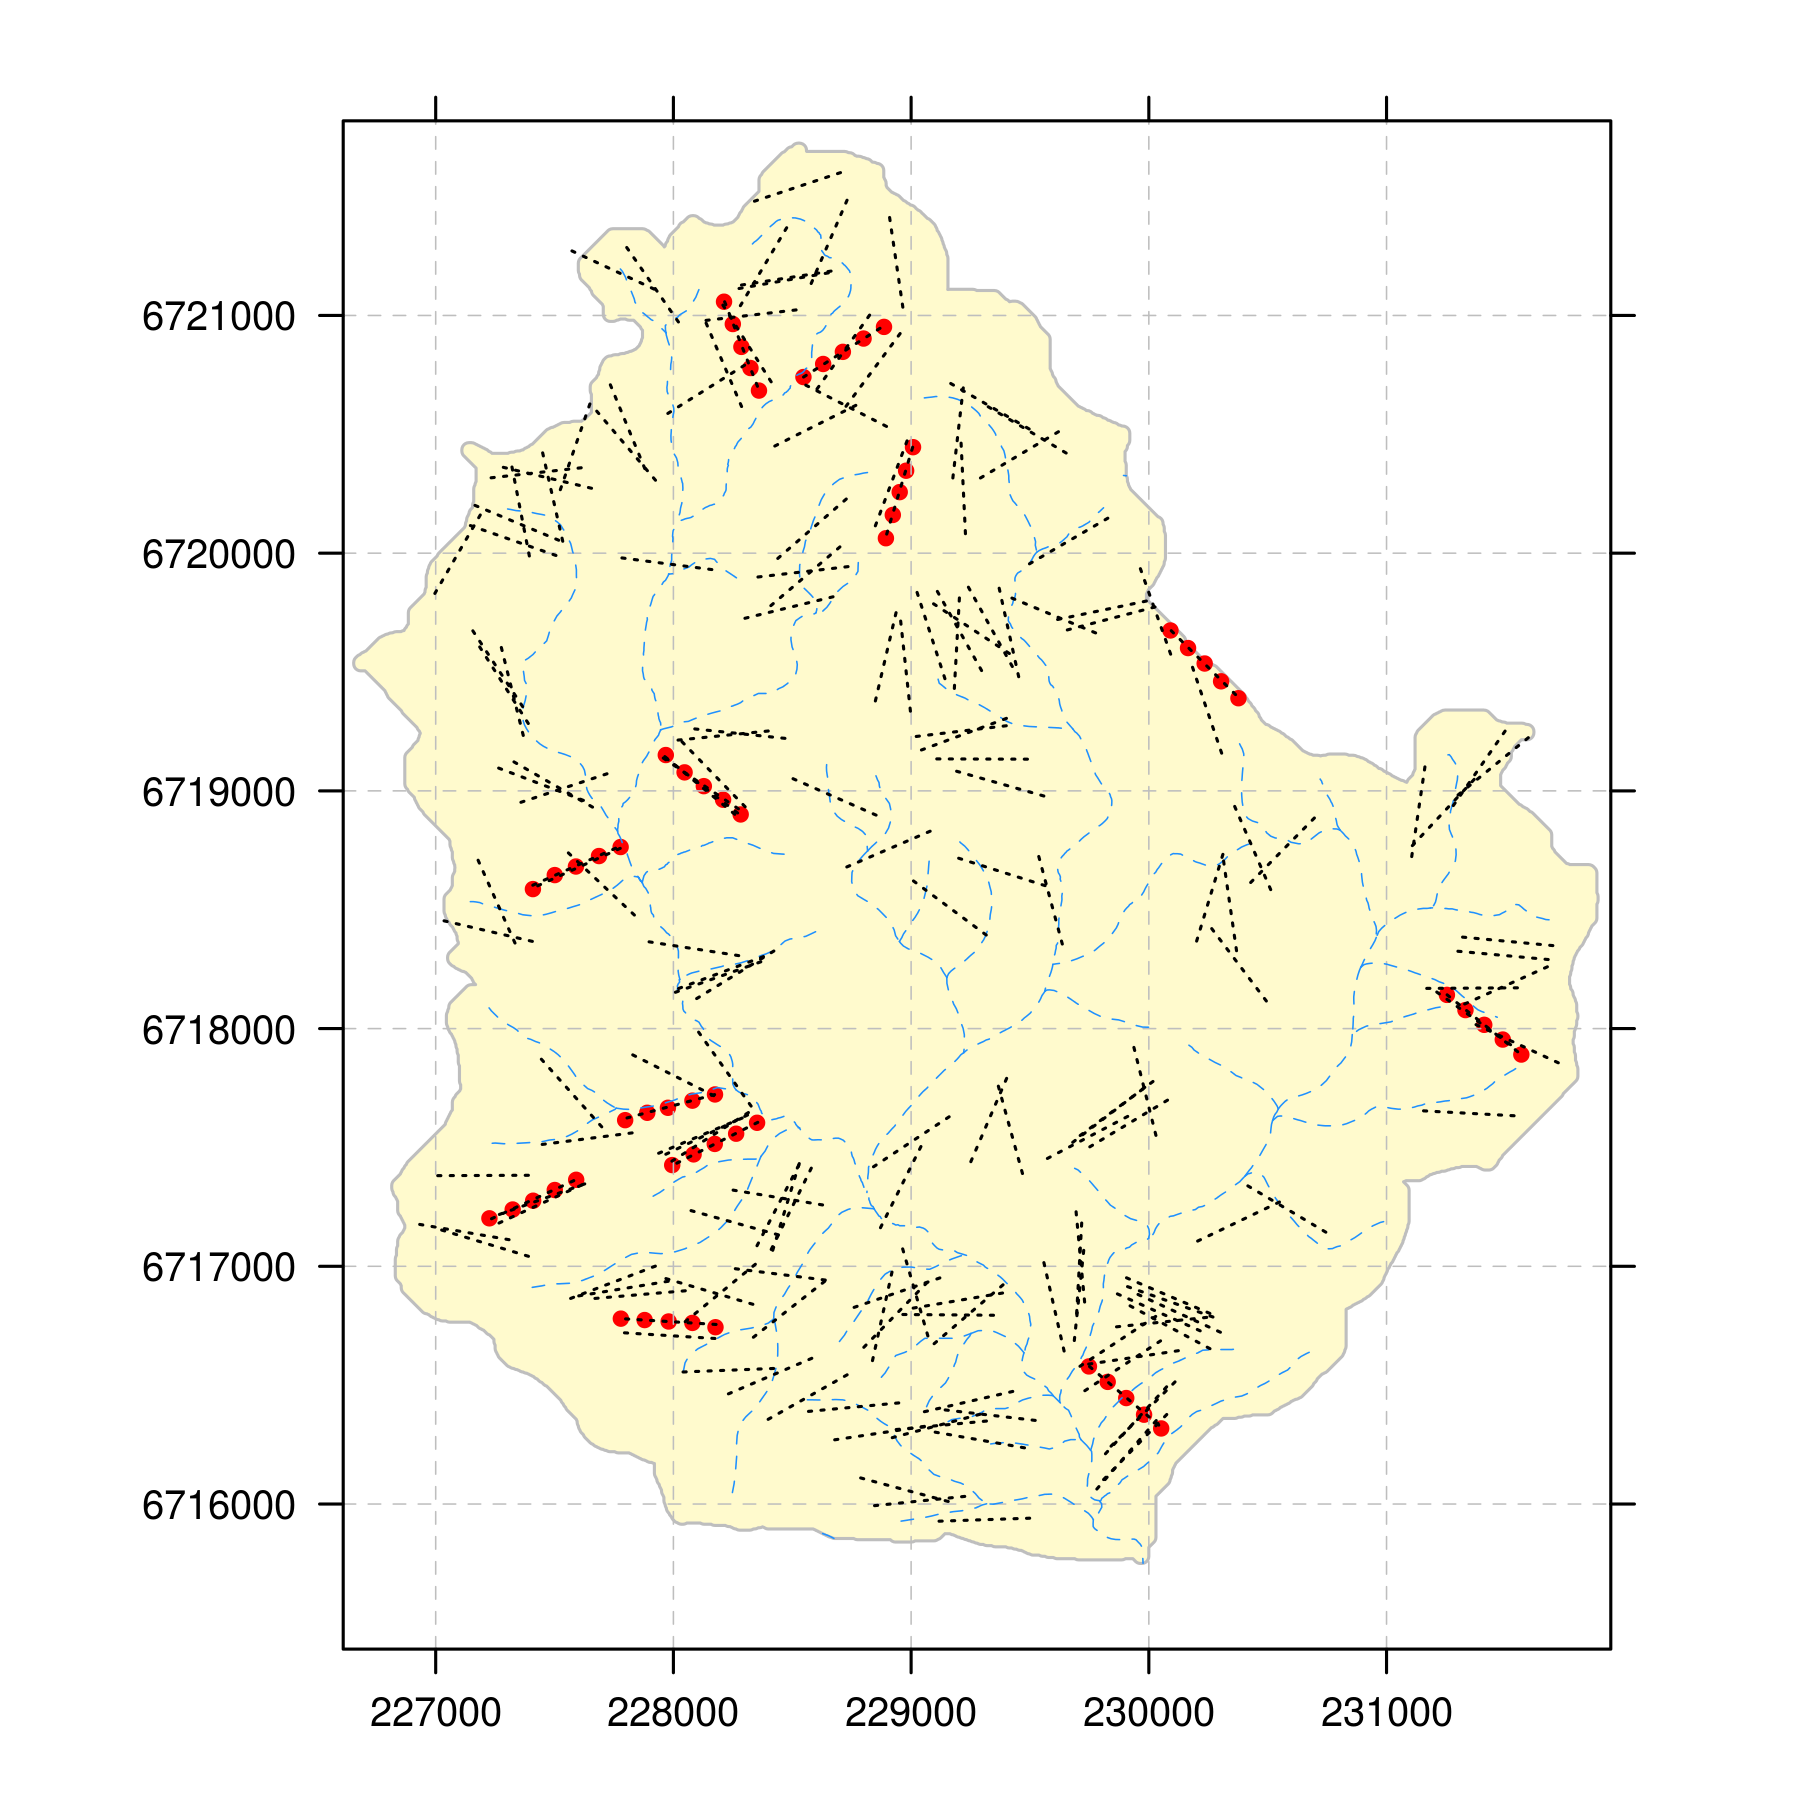
\includegraphics[width=0.90\textwidth]{fig/chap04-subset-II}
\caption[Twelve transects were selected using simple random sampling to yield $n = 60$ validation 
observations]{Three soil spatial modellers manually drew 180 straight transects (black dotted lines) aligned 
in the direction of maximum expected spatial variation of environmental conditions. They avoided locations 
where it was known that geographic barriers or landowners would impede the access to make soil observations. 
Twelve transects were probabilistically selected using simple random sampling to yield $n = 60$ validation 
observations (red solid circles) separated by equidistant intervals of \SI{100}{\metre}. The drainage network 
is shown in the background (blue dashed line) to give an idea of how the location and direction of transects 
is related to terrain features.}
\label{fig:chap04-subset-II}
\end{figure}

Twelve out of the $m = 180$ transects were randomly selected using as many iterations as necessary until 
there were no intersecting transects, and there was at least one transect in each of the three major 
morphostructural units of the DNOS catchment (\textit{Planalto}, \textit{Rebordo do Planalto}, and 
\textit{Depressão Periférica}) (\autoref{chap:chap03}). Finally, $n = 5$ observation locations, separated by 
equidistant intervals of \SI{100}{\metre}, were selected in each transect. Observation locations were named 
with a number in increasing order, following the order in which the observations were made, starting from 
\num{341} (\num{341}--\num{400}).

The location of the observations was identified in the field using a GNSS receiver with a horizontal 
positional error of less than \SI{8}{\metre}. Soil sampling and description was carried out using the same 
procedure used with \emph{Subset I}, except for the fact that a single soil pit was opened within a radius of 
\SI{2}{\m} from the predefined observation location. More accurate geographic coordinates were collected in 
the field using a Differential Global Positioning System (DGPS) with a horizontal positional error of less 
than \SI{1}{\centi\metre}.

\subsection{Subset III}

The third subset ($n = 10$) contains data compiled from the studies of \citet{Pedron2005} and 
\citet{Miguel2010}, specifically from the uppermost A horizon of modal soil profiles (point support) whose 
locations were purposively selected using tacit knowledge after a preliminary area-class soil map had been 
produced and/or the observations included in \emph{Subset I} had been made.

\citet{Pedron2005} and \citet{Miguel2010} aimed at observation locations that they understood as being most 
representative of the soil mapping units depicted in their respective area-class soil maps. A single soil 
sample was taken from each of the described soil horizons and used for laboratory analysis. The resulting 
thickness of the uppermost A horizons varies from \num{12} to \SI{30}{\centi\metre}, with a mean of 
\SI{22.6}{\centi\metre}. Georeferencing was carried using a GNSS receiver with a horizontal positional error 
of less than \SI{8}{\metre} positioned at the observation location. Data are identified in the Santa Maria 
dataset using the same identification that was used in the studies from which they were compiled.

\section{FIELD DESCRIPTION}
\label{sec:chap04-field-description}

Several environmental features were described at the observation locations. This sections present a summary
description of how this description was done, specially for subsets I and II, which have not been documented 
before. For subset III, a thorough explanation of how field description was done is given by 
\citet{Pedron2005} and \citet{Miguel2010}.

Despite the different origins of the datasets, soil sampling and description guidelines are very similar. As 
such, merging field descriptions from subset III with those of subset I and II was easy, rarely requiring 
conceptual translations and adaptations -- this practice is reported when used.

Finally, the code used in the database to identify each of the variables described in the field is presented 
between parenthesis using fixed-width or monospace font.

\subsection{Land Use and Vegetation}

Land use (\texttt{LAND}) was assessed at the time of sampling using data collected in the field. Five land 
uses were identified using nomenclature of \citet{FAO2006} (\autoref{fig:chap04-land}):

\begin{description}
\item[\texttt{animal husbandry}] Native grasslands used for animal husbandry.
\item[\texttt{crop agriculture}] Annual and biannual crop agriculture.
\item[\texttt{forestry}] Plantations of \textit{Eucalyptus spp.} and \textit{Pinus spp.}.
\item[\texttt{native forest}] Primary or secondary native forests.
\item[\texttt{shrubland}] Abandoned areas with predominance of shrub-sized vegetation, known in Brazil as 
\emph{capoeira}.
\end{description}

\begin{figure}[!ht]
\centering
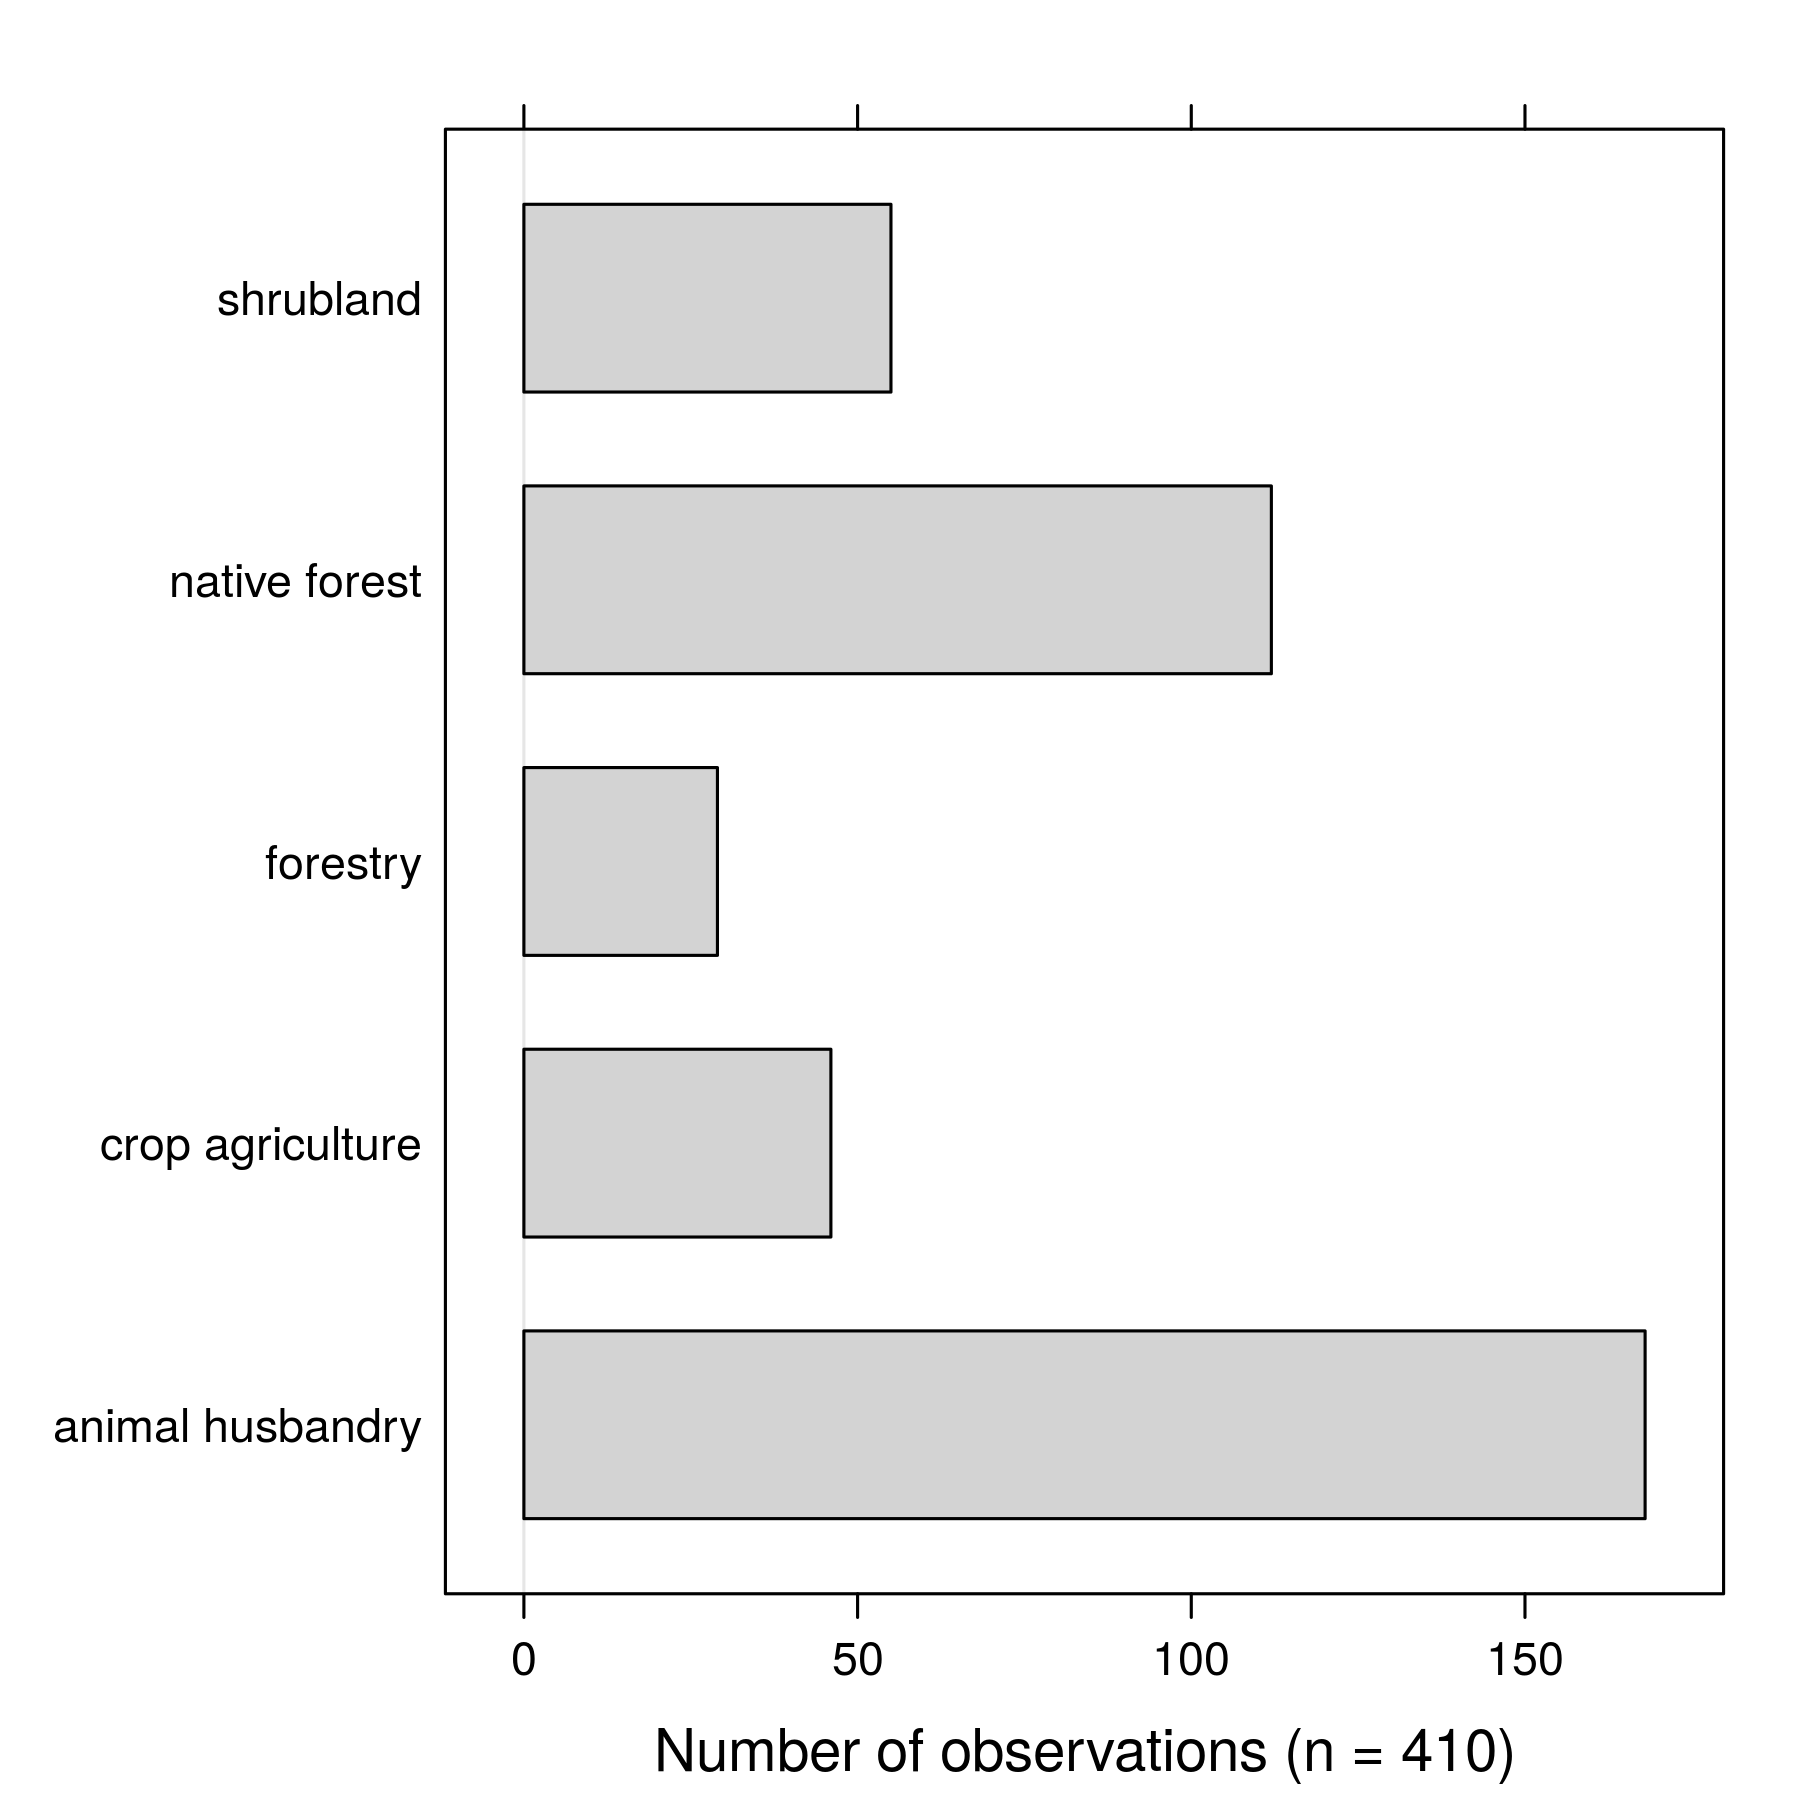
\includegraphics[width=0.60\textwidth]{fig/chap04-land}
\caption[Distribution of land use types in the Santa Maria dataset.]{Distribution of land use types in the 
Santa Maria dataset. Most soil observations were made in areas used for animal husbandry although more that 
half of the area is occupied with native forest (\autoref{sec:chap05-land-use}).}
\label{fig:chap04-land}
\end{figure}

Other land uses are observed in the study area such as human settlements and water bodies 
(\autoref{sec:chap05-land-use}). However, due to access constraints, soil observations were not made in areas 
under these land uses.

\subsection{Geology}

Soil parent material (\texttt{PARENT}) was inferred in the field from direct observation of soil properties 
and local environmental features. Two classes were identified using nomenclature of \cite{FAO2006}:

\begin{description}
\item \texttt{igneous} Soil derived from the \textit{in sutu} weathering of igneous rocks.
\item \texttt{sedimentary} Soil derived from the \textit{in sutu} weathering of sedimentary rocks, or from 
sediments of igneous and/or sedimentary rocks.
\end{description}

Underlying geologic formation (\texttt{GEO}) and lithology (\texttt{LITHO}) were inferred based on soil 
properties and environmental features observed in the field, and on existing area-class soil maps 
(\autoref{sec:chap05-soil-maps}) geologic maps (\autoref{sec:chap05-geo-maps}).

\subsection{Soil Classification}

The most likely taxon (\texttt{TAXON}) of the Brazilian System of Soil Classification (SiBCS) 
\cite{SantosEtAl2013a} was inferred in the field using data obtained from direct observation of soil 
properties (\SI{20}{\centi\metre}-deep soil pits and auger holes down to the diagnostic subsurface horizon or 
bedrock) and local environmental features. These data were then interpreted using the bases and concepts of 
the SiBCS to identify the most likely taxon up to the second taxonomic level of the SiBCS. Further levels of 
the SiBCS were not considered because making any sort of inference would require data that were not observable 
in the field. Eleven taxa were identified (\autoref{fig:chap04-taxon}):

\begin{description}
\item[\texttt{CX}] Cambissolo Háplico. Moderately developed soil.
\item[\texttt{GX}] Gleissolo Háplico. Poorly drained greyish soil with a somewhat constant clay content 
throughout the profile.
\item[\texttt{PA}] Argissolo Amarelo. Soil with significant increase of the clay content with depth, and with 
a yellowish B horizon.
\item[\texttt{PBAC}] Argissolo Bruno-Acinzentado. Soil with significant increase of the clay content with 
depth, and with an upper B horizon slightly darker than the lower B horizons.
\item[\texttt{PV}] Argissolo Vermelho. Soil with significant increase of the clay content with depth, and with 
a reddish B horizon.
\item[\texttt{PVA}] Argissolo Vermelho-Amarelo. Soil with significant increase of the clay content with depth, 
and with a reddish-yellowish B horizon.
\item[\texttt{RL}] Neossolo Litólico. Poorly developed soil.
\item[\texttt{RQ}] Neossolo Quartzarênico. Deep sandy soil derived from sediments.
\item[\texttt{RR}] Neossolo Regolítico. Poorly to moderately developed soil.
\item[\texttt{RY}] Neossolo Flúvico. Poorly developed soil derived from alluvial sediments.
\item[\texttt{SX}] Planossolo Háplico. Poorly drained greyish soil with significant increase of the clay 
content with depth.
\end{description}

\begin{figure}[!ht]
\centering
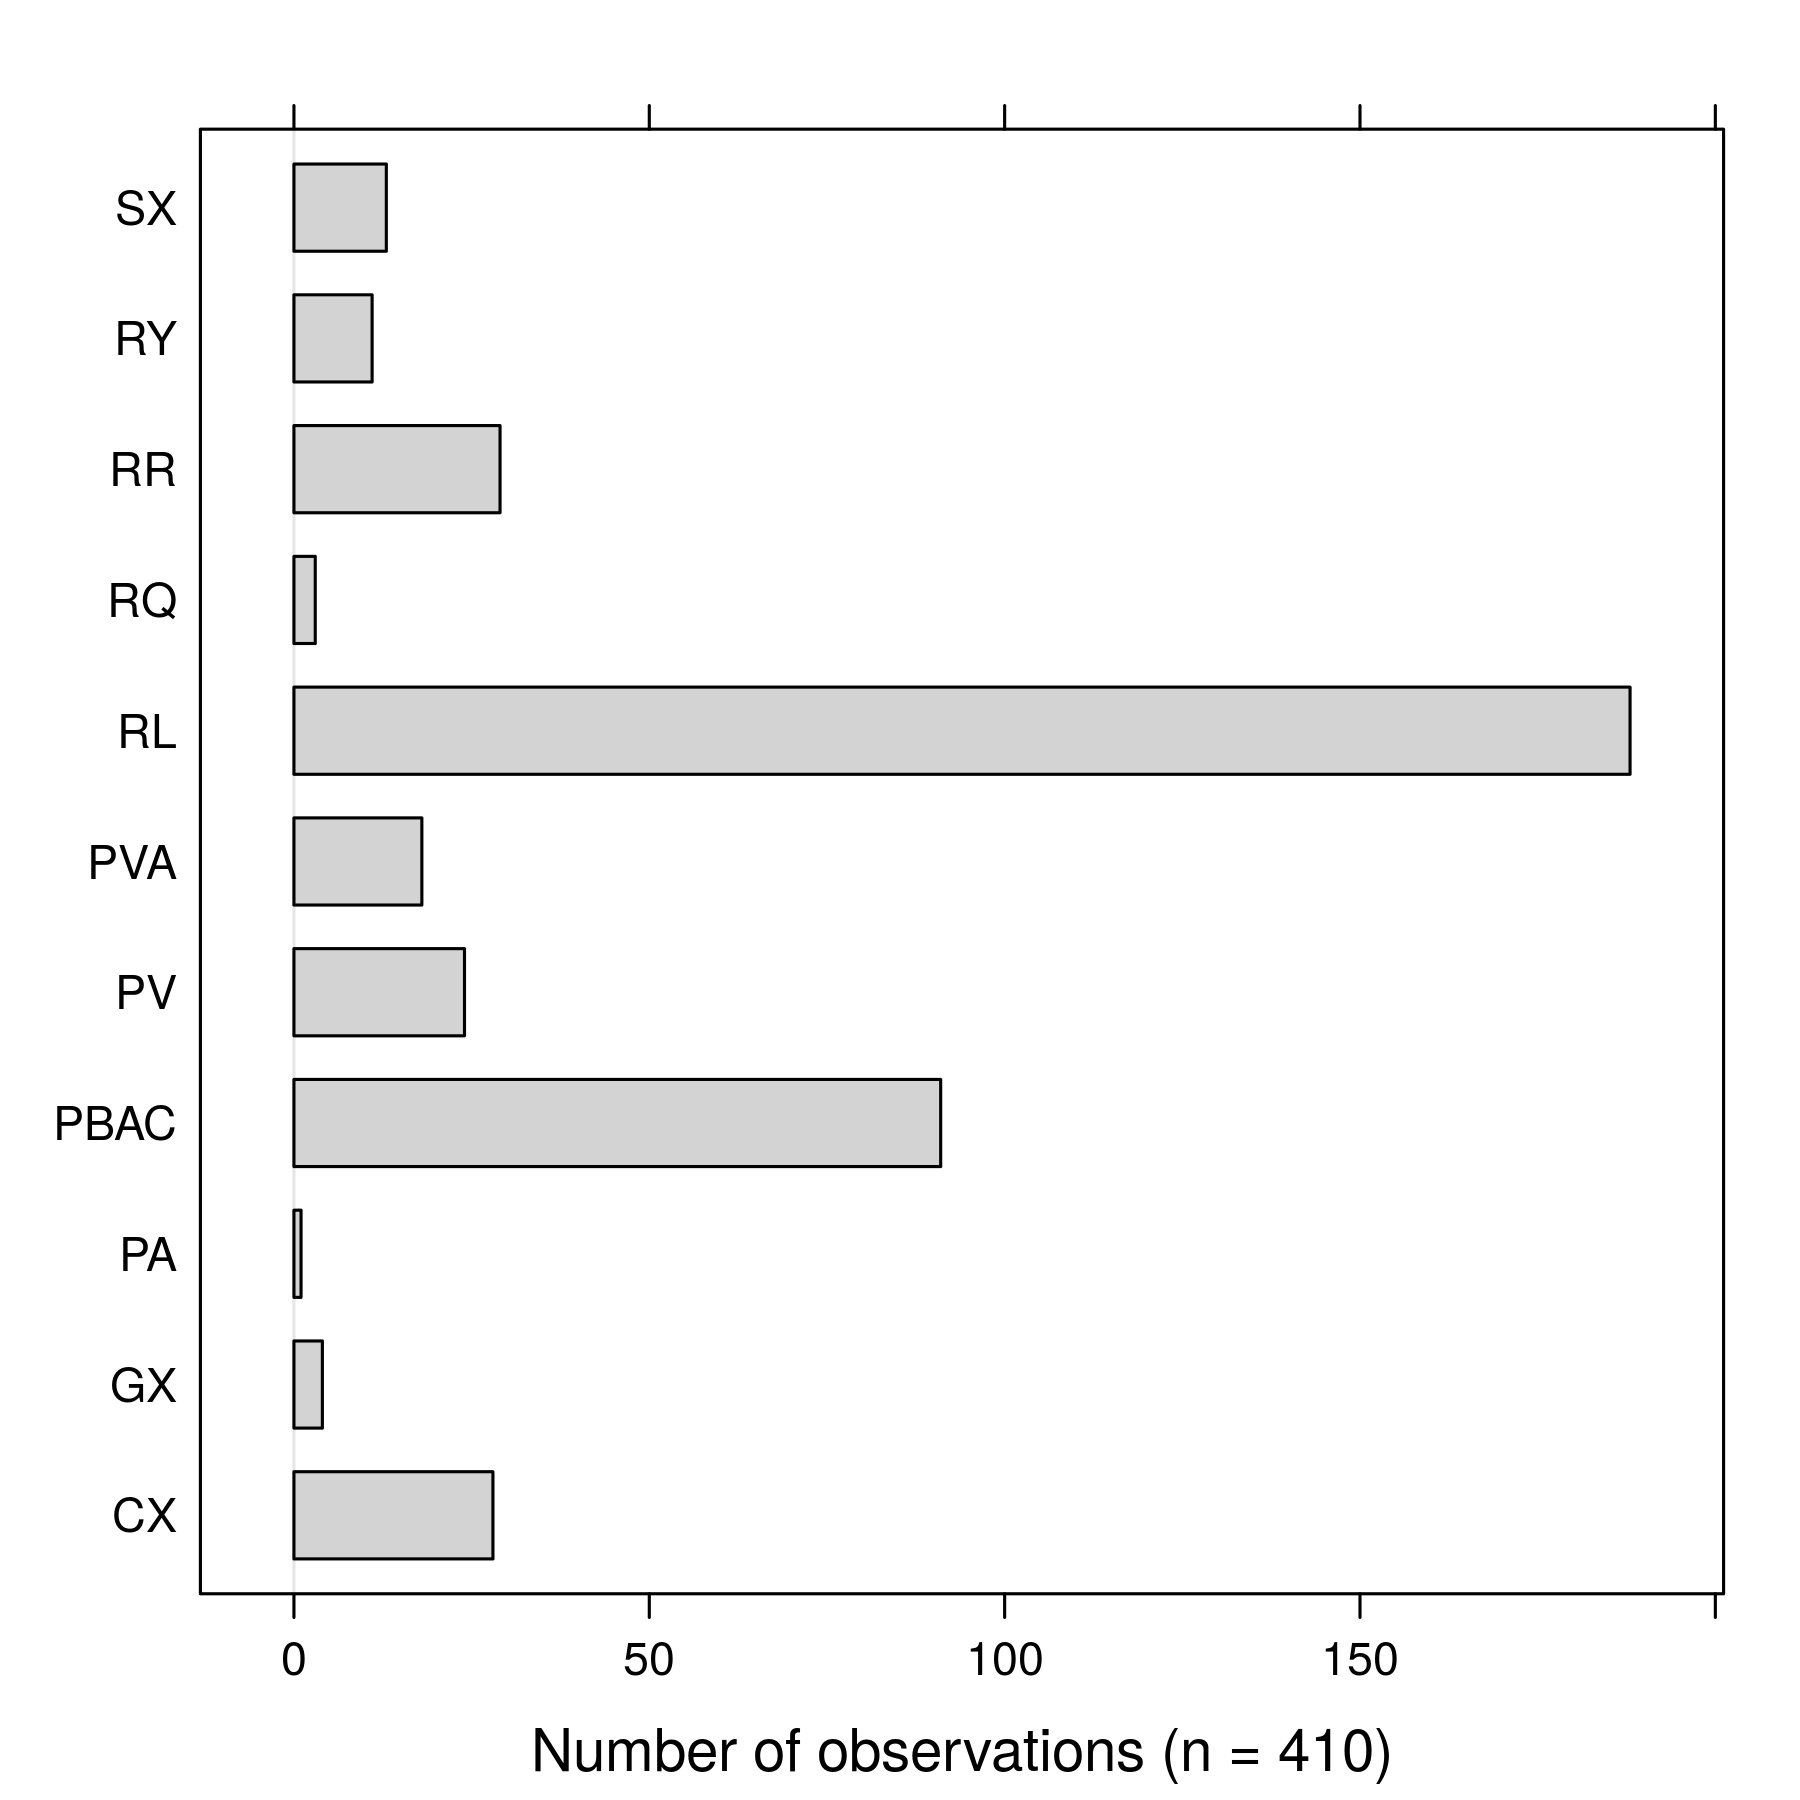
\includegraphics[width=0.60\textwidth]{fig/chap04-taxon}
\caption[Distribution of soil taxa in the Santa Maria dataset.]{Distribution of soil taxa in the Santa Maria 
dataset. Most soil observations were classified as Neossolo Litólico and Argissolo Bruno-Acinzentado. The 
proportions approximately agree with the information conveyed by existing area-class soil maps 
(\autoref{fig:chap05-soil-maps}).}
\label{fig:chap04-taxon}
\end{figure}

\subsection{Slope}

The slope gradient (\texttt{SLOPE}, \si{\percent}) was measured using a clinometer, the observer and target 
being at a constant height above the ground (\autoref{fig:chap04-slope}). The distance between observer and 
target was between \SI{30}{\metre} (dense forests) and \SI{50}{\metre} (open fields).

\begin{figure}[!ht]
\centering
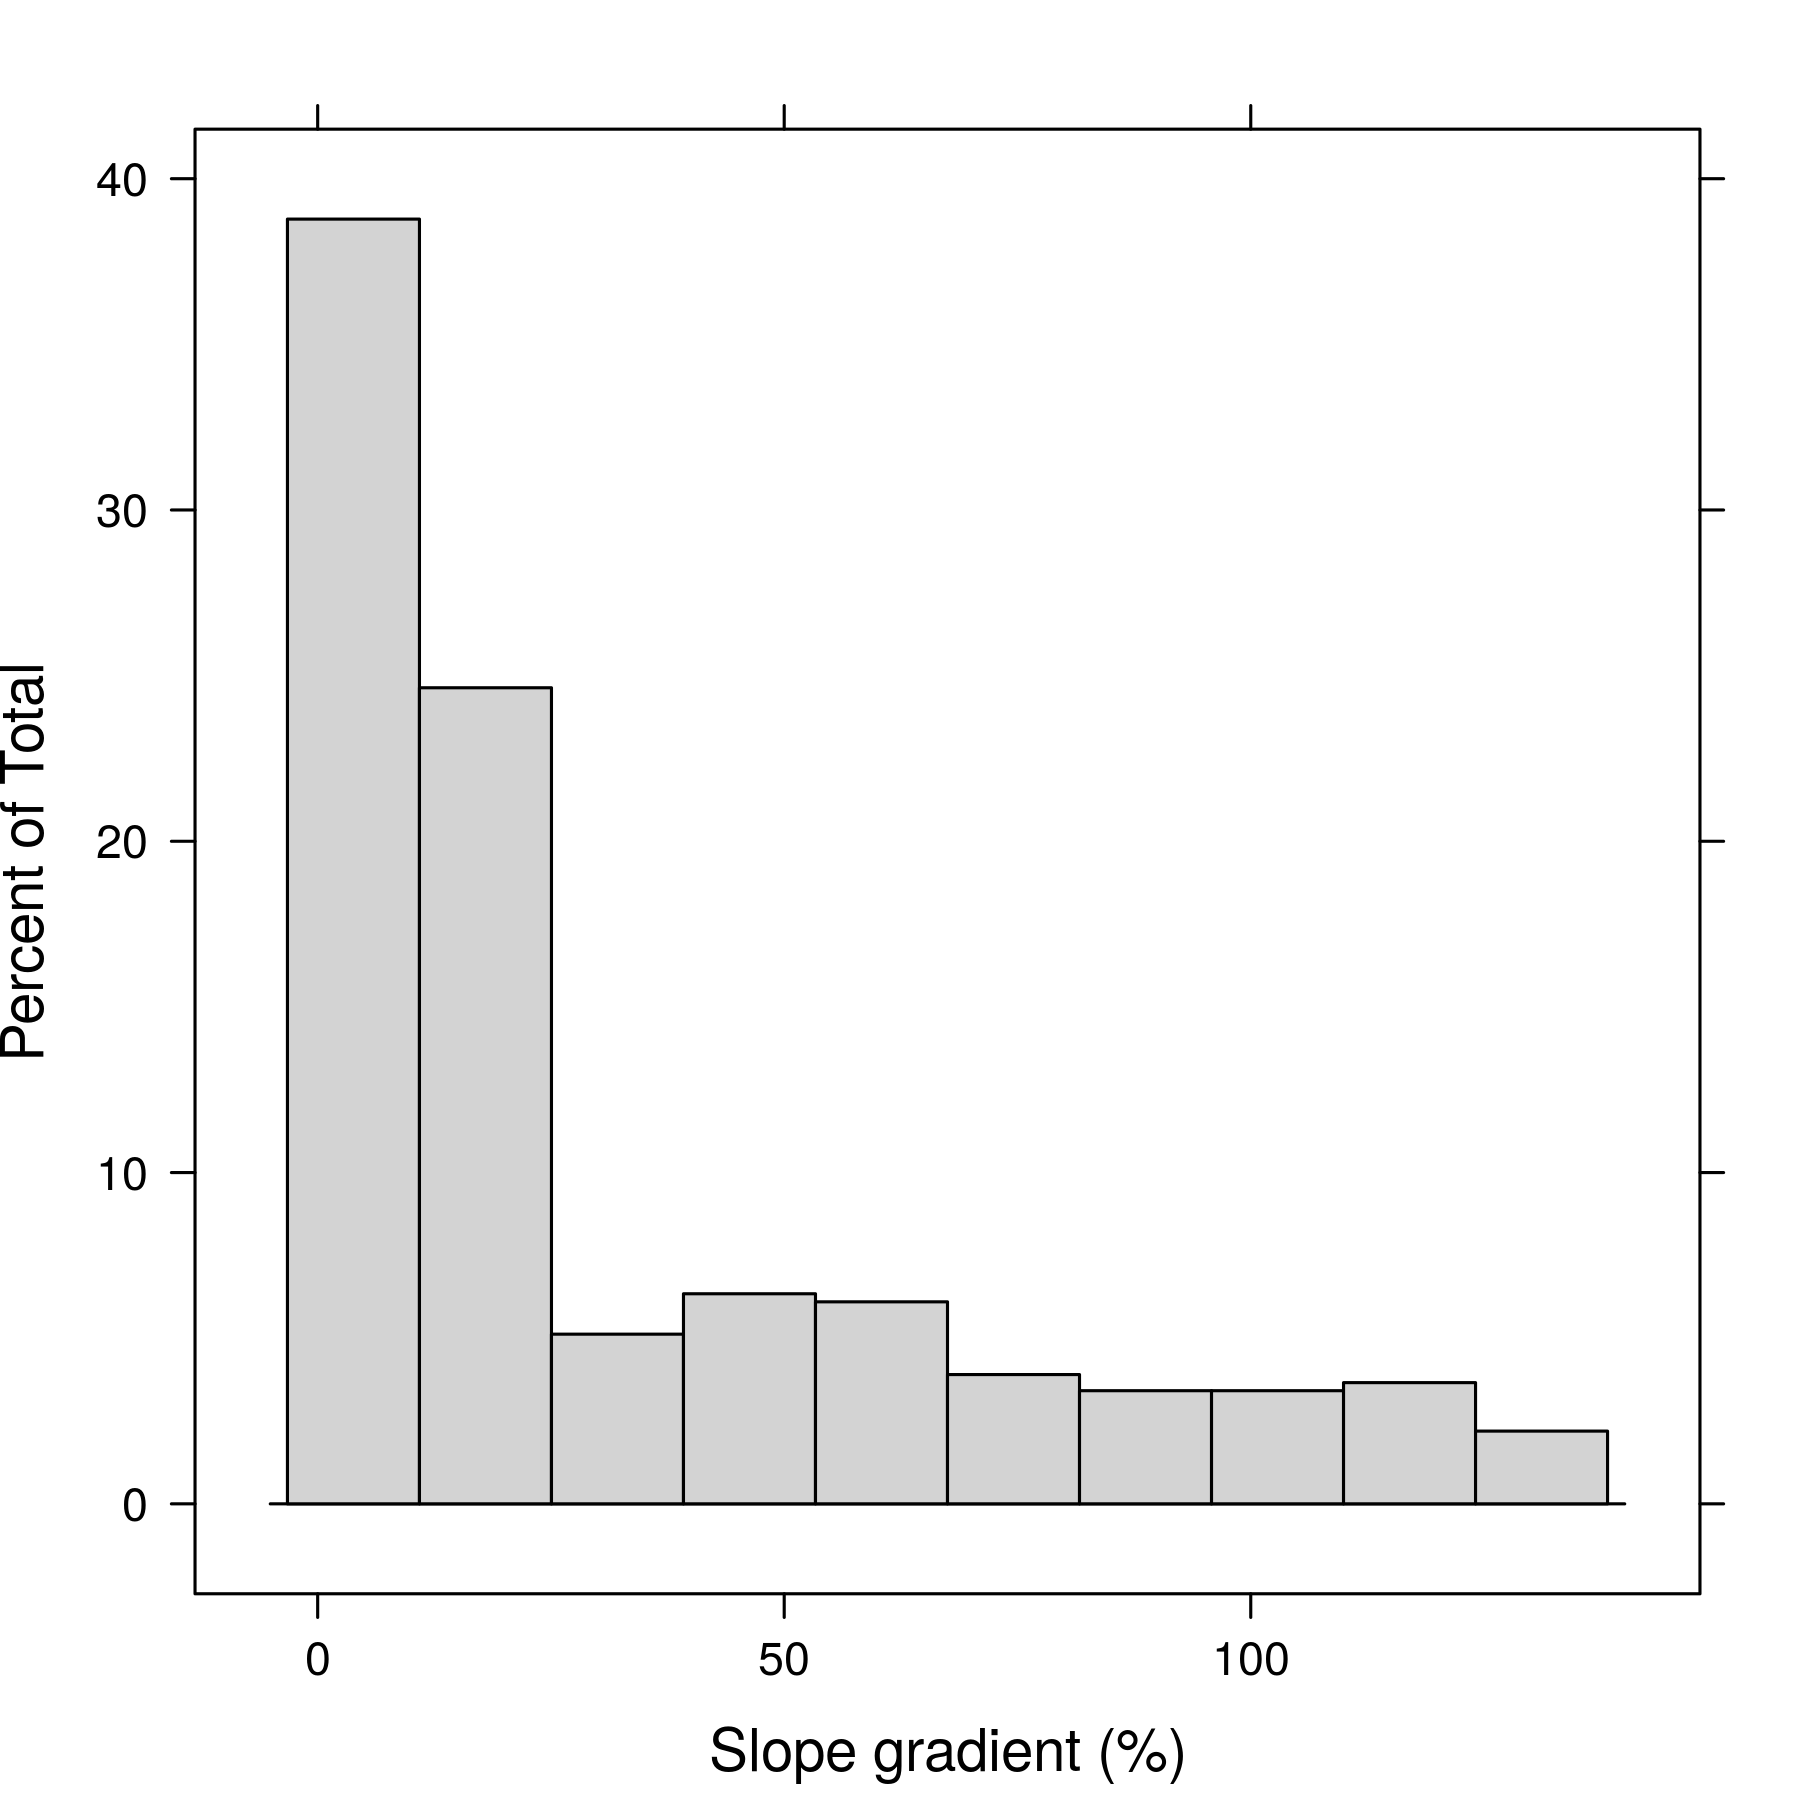
\includegraphics[width=0.60\textwidth]{fig/chap04-slope}
\caption[Distribution of slope gradient in the Santa Maria dataset.]{Distribution of slope gradient in the 
Santa Maria dataset. Most soil observations were made in areas with a slope gradient $\SI{<25}{\percent}$.}
\label{fig:chap04-slope}
\end{figure}

\subsection{Drainage}

Soil drainage status (\texttt{DRAIN}) was inferred visually from soil features observed with an auger using 
the classification scheme proposed by \citet{SantosEtAl2013}. Four drainage classes were identified 
(\autoref{fig:chap04-drain}):

\begin{description}
\item[\texttt{poorly}] Water is removed from the soil so slowly that the profile remains wet for much of the 
time.

\item[\texttt{somewhat poorly}] Water is removed slowly from the soil, so that it remains wet for a 
significant period, but not during most of the year.

\item[\texttt{moderately well}] Water is removed from the soil somewhat slowly, so that the profile remains 
wet for small but significant period of time.

\item[\texttt{well}] Water is removed from the soil with ease but not rapidly.
\end{description}

\begin{figure}[!ht]
\centering
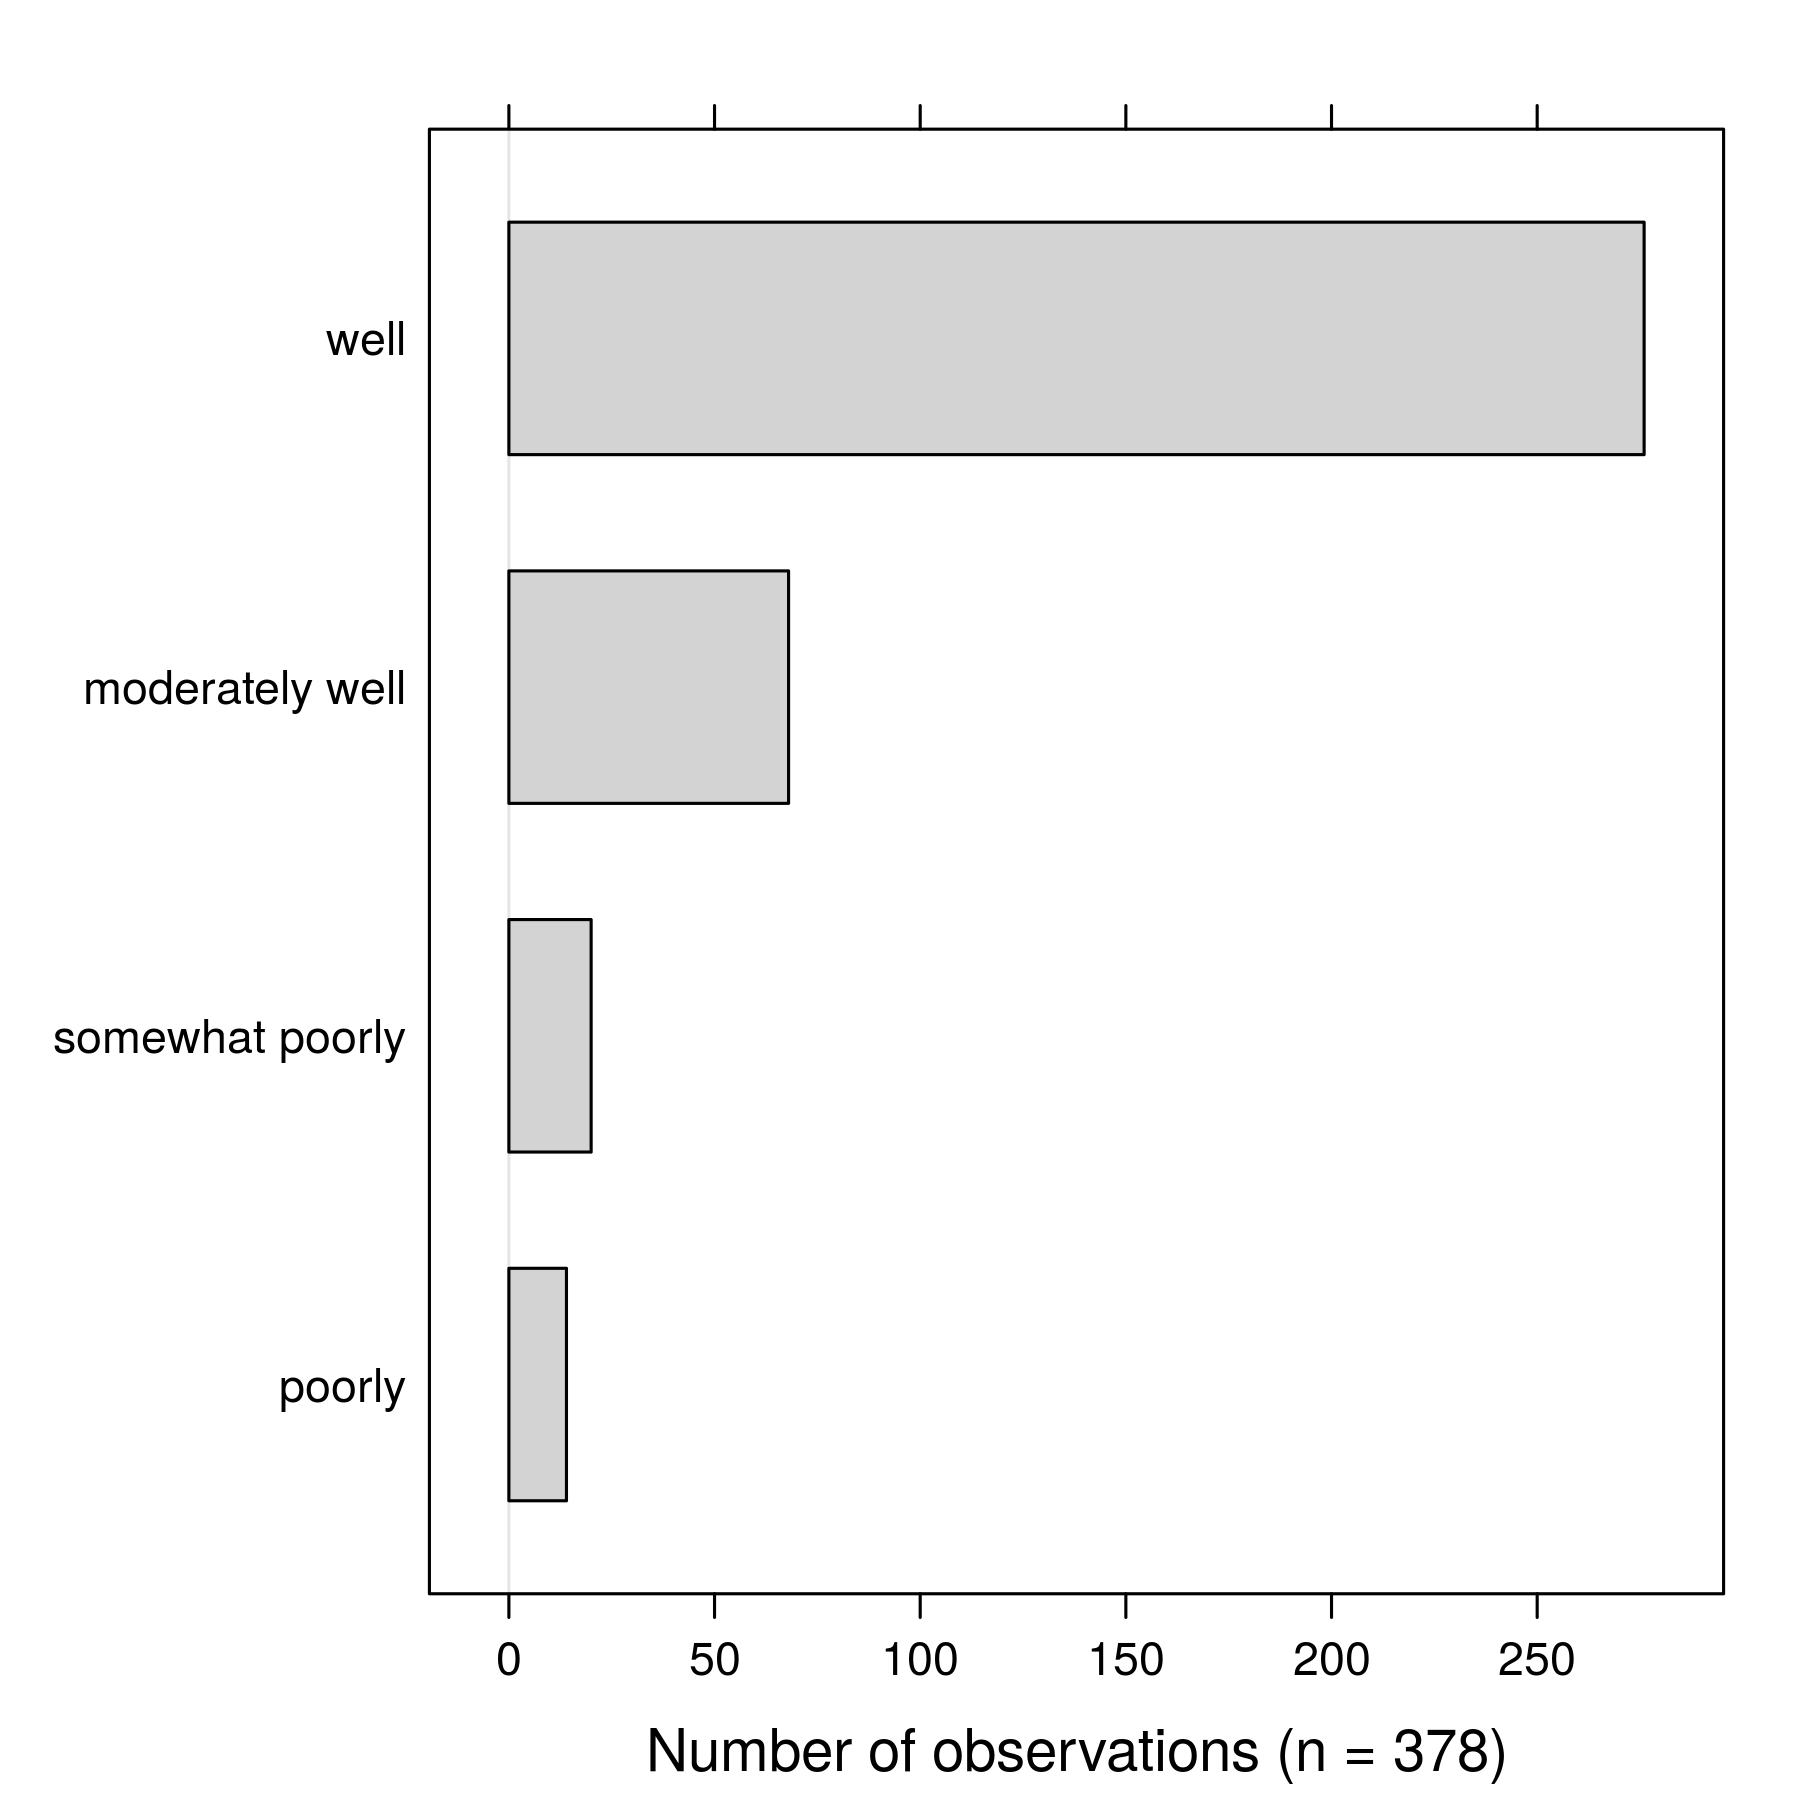
\includegraphics[width=0.60\textwidth]{fig/chap04-drain}
\caption[Distribution of drainage classes in the Santa Maria dataset.]{Distribution of drainage classes in the 
Santa Maria dataset. Most soil observations were made in areas with well drained soil.}
\label{fig:chap04-drain}
\end{figure}

\subsection{Coarse Fragments and Rock Outcrops}

Presence of coarse fragments (\texttt{FRAG}) -- soil material of diameter \SI{>2}{\milli\metre} -- was 
described as a binary variable, that is, a value of \num{1} (one) was annotated when coarse fragments were 
present, and \num{0} (zero) otherwise. The same approach was adopted to describe the presence of rock outcrops 
(\texttt{ROCK}). The quantity of coarse fragments (\texttt{GRAVEL}, \si{\percent}) was estimated visually in 
some observation points.

It is worth noting that the approach employed to describe the presence of coarse fragments and rock outcrops 
is not in line with the standard soil description guidelines currently used in Brazil. The reason for 
recording only their presence/absence is that the actual content was not of primary interest at the time of 
sampling.

\subsection{Canopy}

Soil coverage with vegetation, an estimate of the density of stand or plant cover, (\texttt{CANOPY}) was 
inferred visually in the field using three classes:

\begin{description}
\item[\texttt{low}] \SI{<25}{\percent}
\item[\texttt{medium}] 25--\SI{75}{\percent}
\item[\texttt{high}] \SI{>75}{\percent}
\end{description}

\subsection{Additional Information}

Additional information was recorded at each observation location during the field campaigns. They refer to 
peculiarities of each observation location and were not recorded in a systematic way.

\section{LABORATORY ANALYSIS}
\label{sec:chap04-laboratory}

Several laboratory analysis were performed with the soil samples collected in the DNOS catchment. This 
sections present a summary description of how this analyses were done, specially for subsets I and II, which 
have not been documented before. For subset III, a thorough explanation of how laboratory analyses were done 
is given by \citet{Pedron2005} and \citet{Miguel2010}.

Despite the different origins of the datasets, laboratory analyses protocols are very similar. As such, 
merging the results of laboratory analyses from subset III with those of subset I and II was easy, rarely 
requiring the use of conversion factors -- this practice is reported when used. In all three datasets, soil 
samples were air dried, crushed and passed through a \SI{2}{\milli\metre}-sieve prior to laboratory analyses. 
For datasets I and II, one or more laboratory replicates were used to enable calculating analytical errors.

The same coding standard used with field description variables is used here, i.e. the code used in the 
database is presented between parenthesis using fixed-width or monospace font.

\subsection{Soil Organic Fraction}
\label{sec:chap04-organic}

The soil organic carbon content (\texttt{ORCA}, \si{\gram\per\kilo\gram}) was determined using wet combustion 
\cite{YeomansEtAl1988, Mebius1960, TedescoEtAl1995, ClaessenEtAl1997} (\autoref{fig:chap04-orca}).

% Footnote %%%%%
\def\footsulfochromic{\footnote{See a detailed description of the sulfochromic solution, or chromic acid, at 
\href{http://en.wikipedia.org/wiki/Chromic_acid}{Wikipedia}.}}

Sample aliquots of \num{0.050}--\SI{0.500}{\g} were placed in glass digestion tubes (\SI{80}{\ml}). The 
amount of sample used varied according to the \texttt{ORCA} estimated by visual interpretation of soil colour. 
Every digestion tube received an aliquot of \SI{10}{\ml} of sulfochromic solution\footsulfochromic{} 
[\SI{0.067}{\mole\per\liter} potassium bichromate solution (\ce{K2Cr2O7}) in the presence of concentrated 
sulphuric acid (\ce{H2SO4})] and a small reflux funnel to avoid loss of reagent during digestion. A digestion 
block with capacity for \num{40}~samples was used: \num{36}~tubes with soil sample plus \num{3}~tubes with 
blank plus \num{1}~tube with \ce{H2SO4} and a thermometer for temperature check. Digestion at 
\SI{150}{\celsius} last \SI{30}{\minute}. Three blanks were prepared and set aside at room temperature to 
estimate the loss of reagent due to heat in the digestion block.

After digestion the tubes were set aside at room temperature to cool down. Next, the solution was transferred 
to Erlenmeyer flasks (\SI{250}{\ml}) with \SI{60}{\ml} of distilled water and \SI{2}{\ml} of concentrated 
orthophosphoric acid [\ce{H3PO4}] and \num{3}~drops of \SI{1}{\percent}~diphenylamine. The solution was 
titrated using \SI{0.1}{\mole\per\liter} ammonium ferrous sulphate (\ce{FeSO4(NH4)2 * 6H2O}) until persistent 
green colour. The results were multiplied by \num{1.11} to correct the estimated soil organic carbon content 
to the standard analytical method (dry combustion).

\begin{figure}[!ht]
\centering
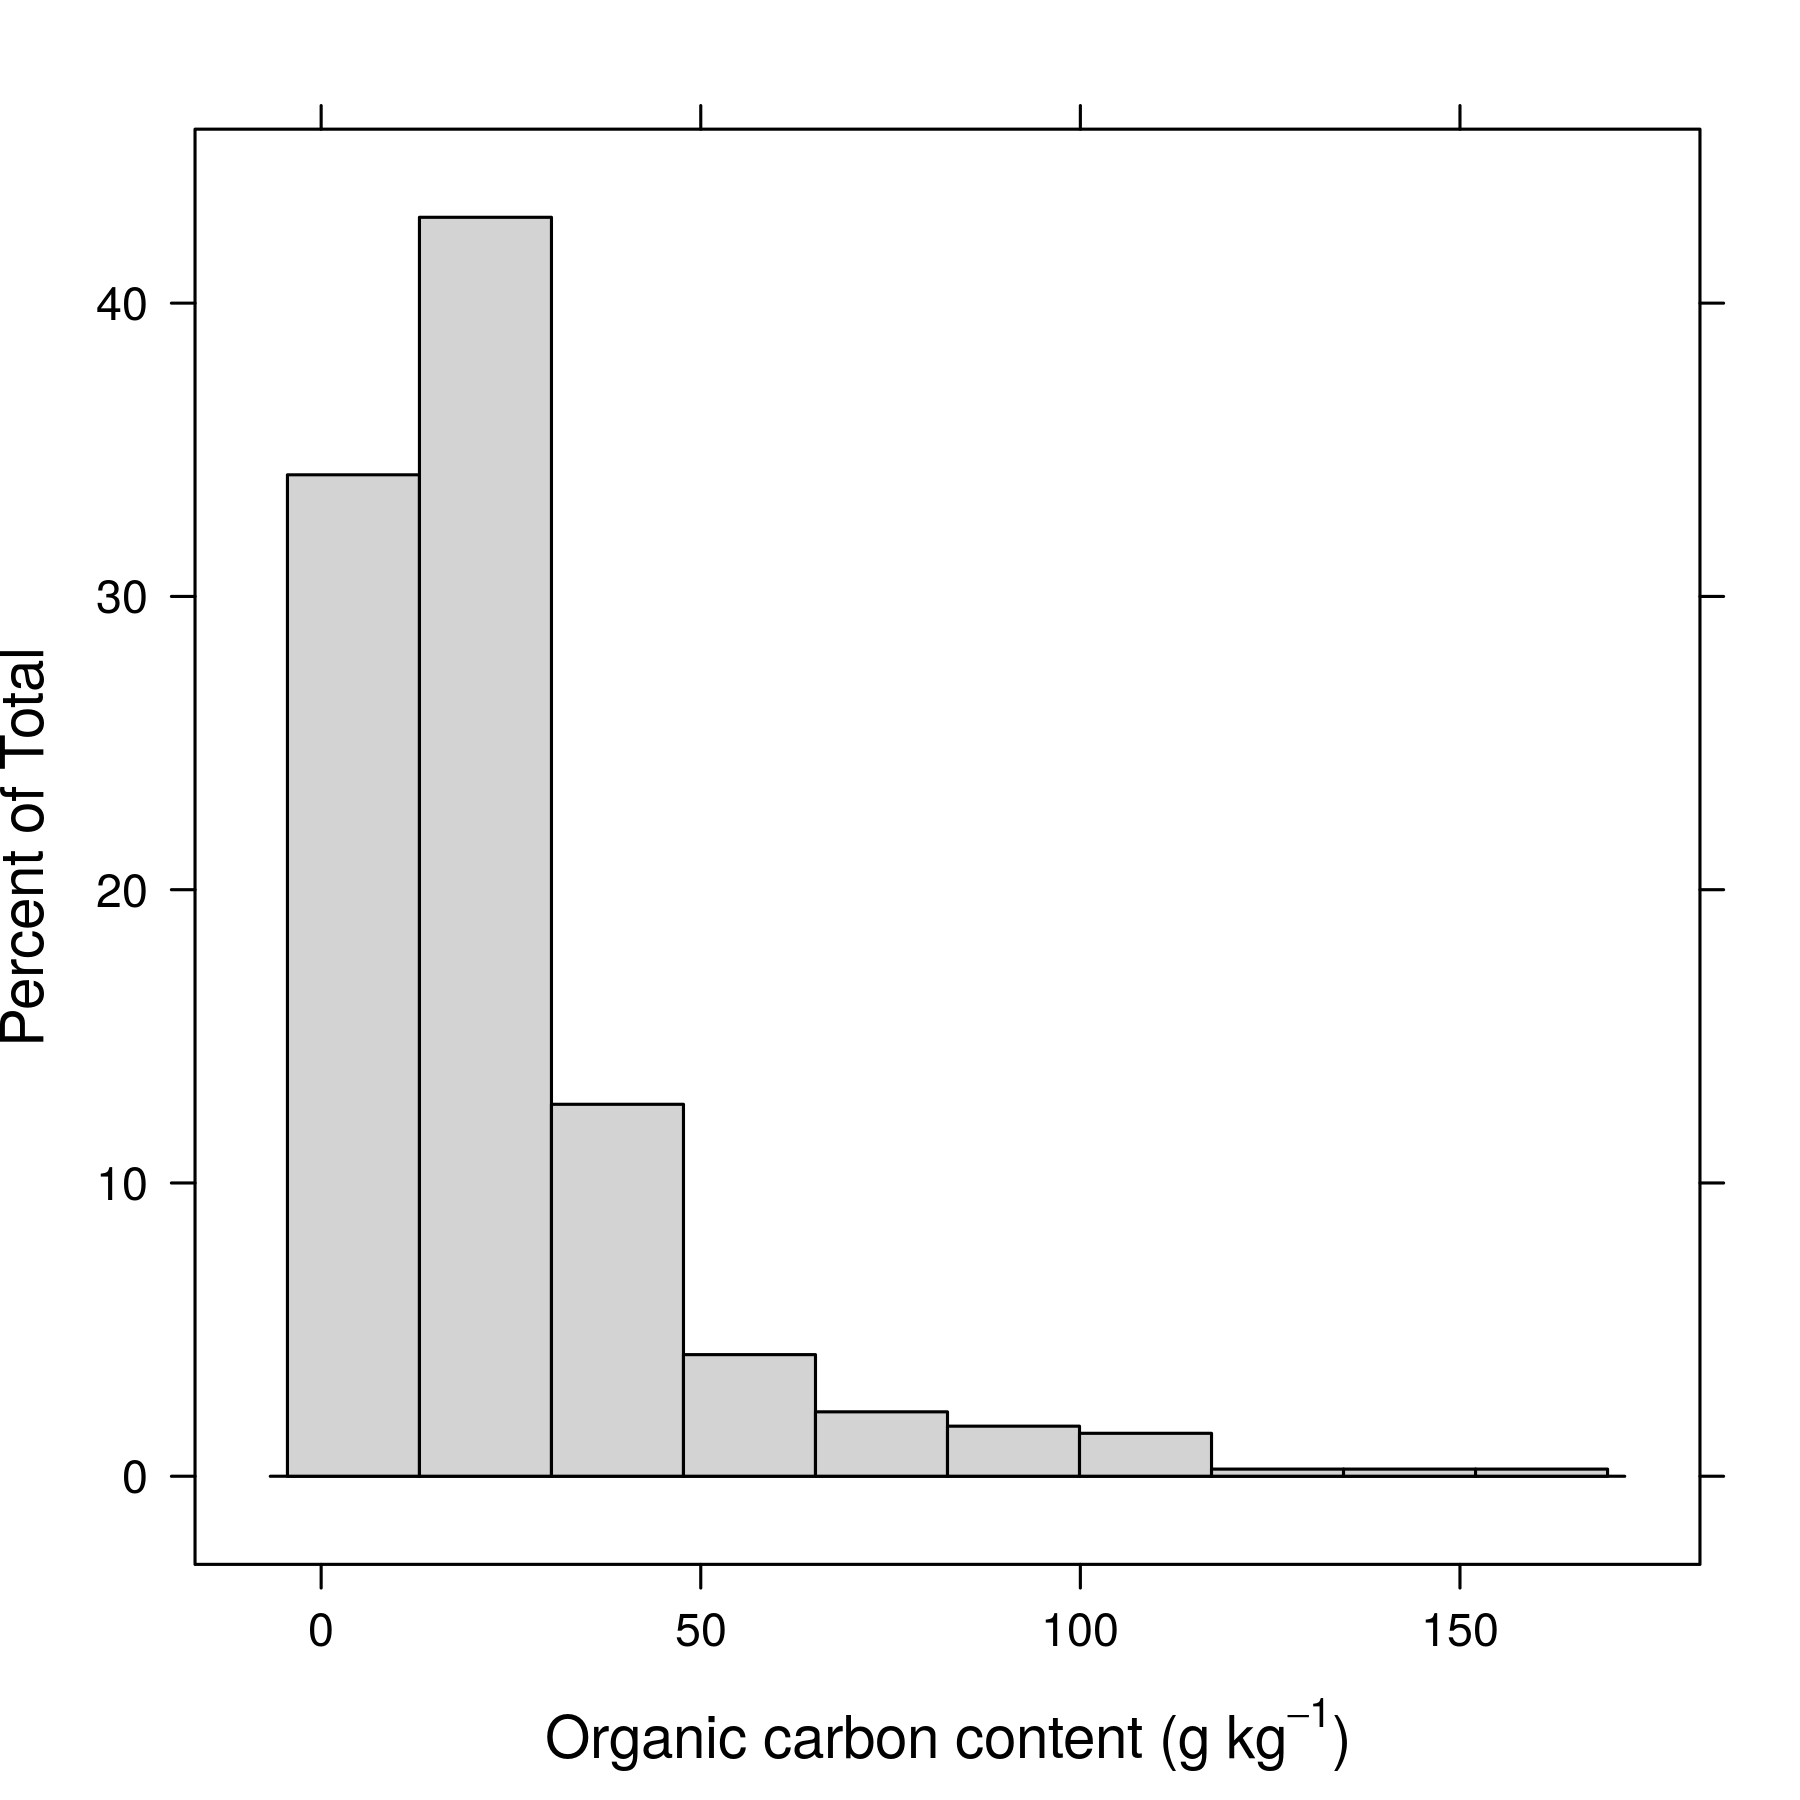
\includegraphics[width=0.60\textwidth]{fig/chap04-orca}
\caption[Distribution of organic carbon content in the Santa Maria dataset.]{Distribution of organic carbon 
content (\si{\gram\per\kilo\gram}) in the Santa Maria dataset.}
\label{fig:chap04-orca}
\end{figure}

Observations compiled from \citet{Pedron2005} had their soil organic matter content determined instead of the 
soil organic carbon content. Sample aliquots of \SI{2.5}{\ml} were placed in Erlenmeyer flasks (\SI{50}{\ml}). 
Every Erlenmeyer flask received an aliquot of \SI{15}{\ml} of \SI{0.067}{\mole\per\liter} sulfochromic 
solution (\ce{Na2Cr2O7 + H2SO4}). The flasks were heated in a water bath at 75--\SI{80}{\celsius} during 
\SI{30}{\minute} and shaken for \SI{5}{\minute}. A water aliquot of \SI{15}{\ml} was added to the flask and 
let overnight (15--\SI{18}{\hour}).

In the next day, an aliquot of \SI{3.0}{\ml} was sampled to a small plastic cup with \SI{3.0}{\ml} of 
distilled water. The absorbency of the supernatant was measured at \SI{645}{\nano\metre}. The estimated soil 
organic matter content was transformed to soil organic carbon content assuming that \SI{58}{\percent} of the 
soil organic matter is composed of organic carbon. The resulting transformed \texttt{ORCA} value was assumed 
to be equivalent to soil organic carbon content measured using the standard analytical method (dry 
combustion). The results are expressed using a volume-basis and were converted to a mass-basis using a 1:1 
relation because the mass of the sample aliquot used in the analyses is unknown.

\subsection{Particle Size Analysis}
\label{chap:chap04-granulometry}

% Footnote %%%%%
\def\footsuzuki{\footnote{As far as I know, a comprehensive description of this method has not been published 
so far, neither in Portuguese nor in English. You can visit the homepage of the Soil Physics Laboratory of the 
Universidade Federal de Santa Maria at \url{https://coral.ufsm.br/fisicadosolo/} to get more information about 
the method or contact their developers.}}

Particle size analysis was performed using the pipette method (\texttt{CLAY}, \SI{<0.002}{\mm}, 
\si{\gram\per\kilo\gram}), with the sand fraction (\texttt{SAND}, 0.053--\SI{2}{\mm}, 
\si{\gram\per\kilo\gram}) determined by wet sieving, and the silt fraction (\texttt{SILT}, 
0.002--\SI{0.053}{\mm}, \si{\gram\per\kilo\gram}) calculated by difference \cite{ClaessenEtAl1997}. The 
analytical procedure includes adaptations\footsuzuki{} of the method of the Soil Conservation Service of the 
United States Department of Agriculture \cite{UnitedStates1972} made by the Soil Physics Laboratory of the 
\textit{Universidade Federal de Santa Maria} \cite{SuzukiEtAl2004, SuzukiEtAl2004a}.

Before particle size analysis, all soil samples with organic matter content \SI{>5}{\percent} -- estimated 
assuming that \SI{58}{\percent} of the soil organic matter is composed of organic carbon -- were submitted to 
oxidative treatment with hydrogen peroxide (\ce{H2O2}). For this end, an aliquot of \SI{20}{\g} of soil was 
placed in a \SI{1000}{\ml} Beaker, to which \SI{15}{\ml} of distilled water and 5--\SI{15}{\ml} of 
\SI{30}{\percent} \ce{H2O2} were added -- the larger the \texttt{ORCA}, the smaller the quantity of \ce{H2O2} 
added to avoid loss of material due to the strong frothing that usually takes place during the first addition 
of \ce{H2O2}. The mixture was homogenized and covered with a watch glass and allowed to stand for 
\SI{12}{\hour}, when another 5--\SI{15}{\ml} of \ce{H2O2} was added. The addition of 5--\SI{15}{\ml} of 
\ce{H2O2} continued at approximately regular intervals of \SI{6}{\hour} until the mixture did not present any 
more effervescence (frothing). The Beaker was transferred to hot plate at a temperature of \SI{50}{\celsius} 
to evaporate the excess water and remove any remaining \ce{H2O2}. All \ce{H2O2}-treated soil material was 
transferred quantitatively to a tared \SI{100}{\ml} glass container and put to dry overnight in an oven at 
\SI{45}{\celsius}. When the soil material was completely dry, the glass container was transferred to a 
desiccator chamber where it was let to cool for \SI{30}{\minute}. Then, the glass container was weighted with 
\SI{0.001}{\g} accuracy to estimate quantity of soil material remaining after the \ce{H2O2} treatment.

For particle size analysis, a sample aliquot of \SI{20}{\g} (or approximately \SI{20}{\g} when the material 
was submitted to oxidative treatment with \ce{H2O2}) was placed in a \SI{100}{\ml} glass container (height: 
\SI{10.5}{\cm}; diameter: \SI{2.75}{\cm}; weight: \SI{85}{\g}). Two nylon spheres with a diameter of 
\SI{1.71}{\cm} and weighting \SI{3.04}{\g} (density: \SI{1.11}{\g\per\cm\cubic}) were added to act as physical 
disaggregating agents. Then, an aliquot of \SI{10}{\ml} of \SI{1}{\mole\per\liter} sodium hydroxide 
(\ce{NaOH}) solution was added to act as chemical dispersing agent along with \SI{40}{\ml} of distilled water. 
The glass container was closed with a plastic cap, manually shaken for \SI{10}{\second}, and placed in a 
horizontal mechanical shaker with capacity for \num{85}~samples. The suspension was left to stand overnight 
(\SI{10}{\hour}). In the next day the suspension was submitted to horizontal mechanical agitation during 
\SI{4}{\hour} at \si{120} cycles per minute.

\begin{figure}[!ht]
\centering
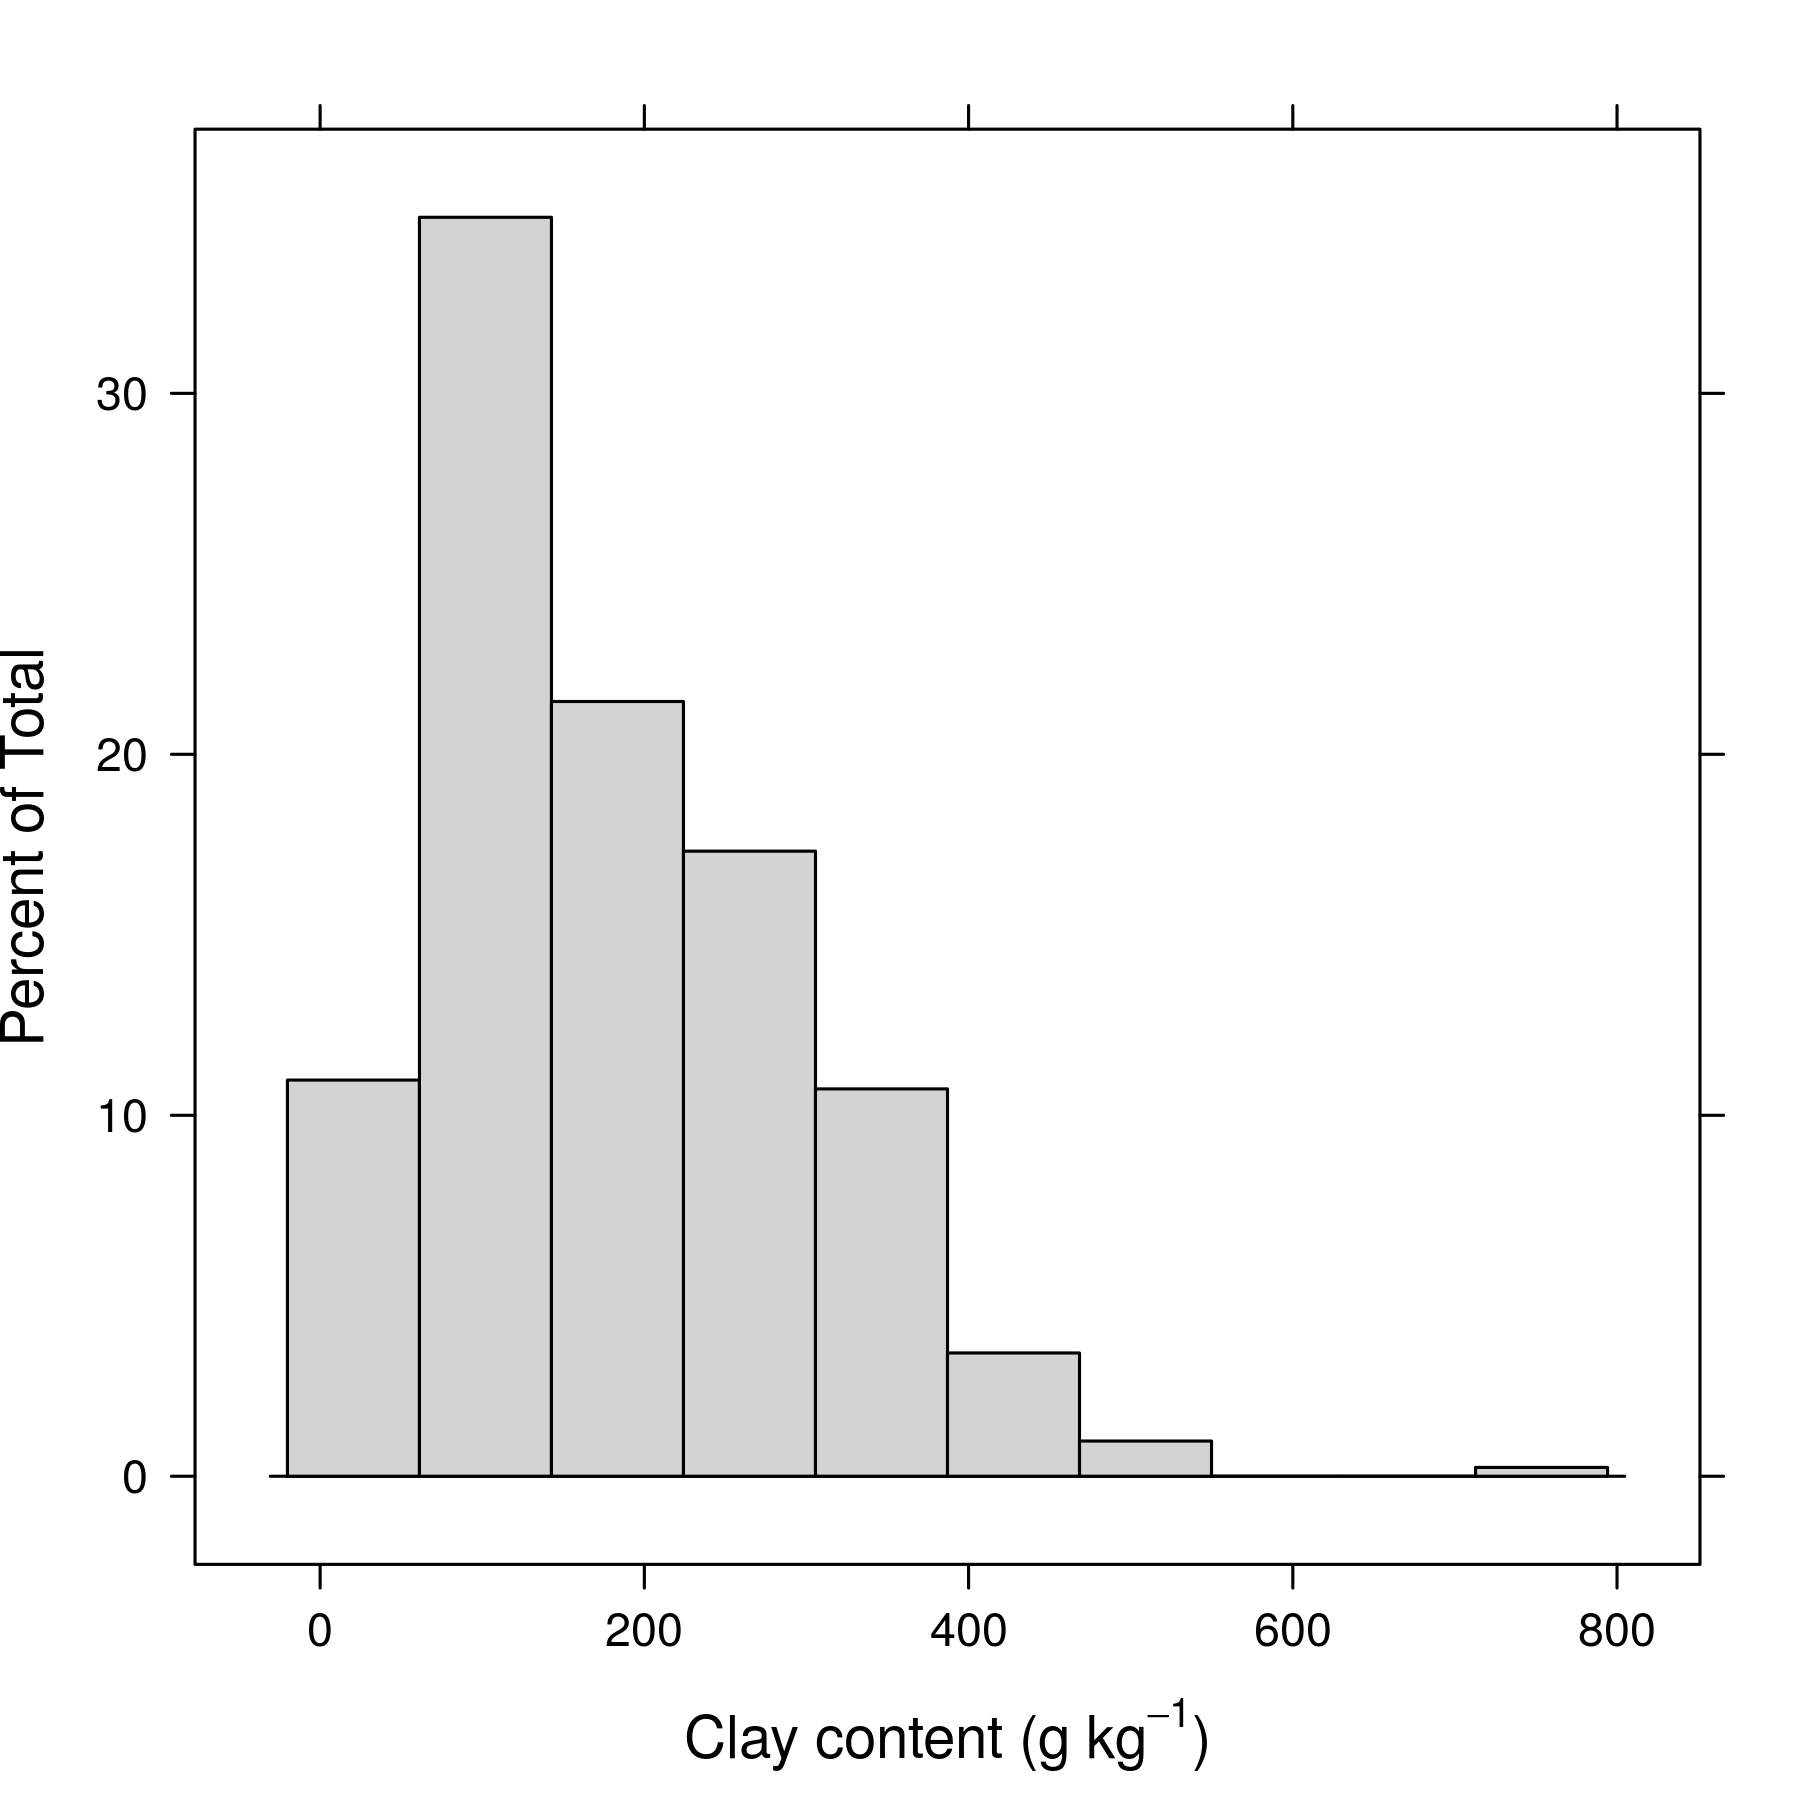
\includegraphics[width=0.60\textwidth]{fig/chap04-clay}
\caption[Distribution of clay content in the Santa Maria dataset.]{Distribution of clay content 
(\si{\gram\per\kilo\gram}) in the Santa Maria dataset.}
\label{fig:chap04-clay}
\end{figure}

After horizontal agitation, the suspension was poured in a plastic graduated cylinder with capacity for 
\SI{1000}{\ml} using a glass funnel and a metal sieve to hold the two nylon spheres. The suspension in the 
graduated cylinder was completed to \SI{1000}{\ml} and homogenized using a hand stirrer (\SI{30}{\second}). 
The suspension was allowed to stand on a vibration-free table to settle the clay fraction (\SI{<0.002}{\mm}) 
to a depth of \SI{5}{\cm}. The settling time needed was calculated using the Stokes’ law with the temperature 
measured in a graduated cylinder filled with distilled water. After settling, an aliquot of \SI{50}{\ml} of 
the suspension was collected at a depth of \SI{5}{\cm} using a hand volumetric pipette. The aliquot was 
transferred to a tared moisture Beacker and put to dry overnight at \SI{105}{\celsius}. When the material was 
completely dry, the Beacker was transferred to a desiccator chamber where it was let to cool for 
\SI{30}{\minute}. Then, the Beacker was weighted with \SI{0.001}{\g} accuracy to estimate \texttt{CLAY} 
(\autoref{fig:chap04-clay}).

The suspension remaining in the plastic graduated cylinder after the \SI{50}{\ml}-aliquot had been collected 
was passed through a \SI{0.053}{\mm} sieve. The material retained in the sieve was washed thoroughly with 
water tap. The remaining material was quantitatively transferred to a tared moisture Beacker and put to dry 
overnight at \SI{105}{\celsius}. When the material was completely dry, the Beacker was transferred to a 
desiccator chamber where it was let to cool for \SI{30}{\minute}. Then, the Beacker was weighted with 
\SI{0.001}{\g} accuracy to estimate \texttt{SAND}.

%The sand fraction was separated into five size classes:
%
%\begin{itemize}
%\item \SIrange{1.00}{2.00}{\milli\metre}: very coarse sand;
%\item \SIrange{0.50}{1.00}{\milli\metre}: coarse sand;
%\item \SIrange{0.25}{0.50}{\milli\metre}: median sand;
%\item \SIrange{0.106}{0.25}{\milli\metre}:fine sand;
%\item \SIrange{0.053}{0.106}{\milli\metre}: very fine sand.
%\end{itemize}

% The clay fraction (\textless0.002~mm) was initially determined by the pipette method without any 
% pretreatment. A 1~mol~L$^{-1}$ NaOH solution was used as the dispersing agent, with the addition of two 
% nylon spheres as disaggregating agent plus horizontal mechanical agitation during 4~hours 
% \cite{SuzukiEtAl2004}.

% A propor{\c{c}}{\~{a}}o da fra{\c{c}}{\~{a}}o argila dispersa em {\'{a}}gua foi determinada conforme 
% descrito acima para a fra{\c{c}}{\~{a}}o argila total. A diferen{\c{c}}a {\'{e}} que n{\~{a}}o foi usado o 
% agente dispersante (NaOH) e o agente desagregante (esferas de nylon) \cite{ClaessenEtAl1997}.

\subsection{Soil Density}
\label{chap:chap04-bude}

% TODO: Provide a more detailed description of how this is done.
The bulk soil density (\texttt{BUDE}, \si{\mega\gram\per\cubic\metre}) at the soil surface was determined 
using the core method with a metallic ring (height: \SI{3}{\centi\metre}; diameter: \SI{5}{\centi\metre}) 
\cite{ClaessenEtAl1997} (\autoref{fig:chap04-bude}).

\begin{figure}[!ht]
\centering
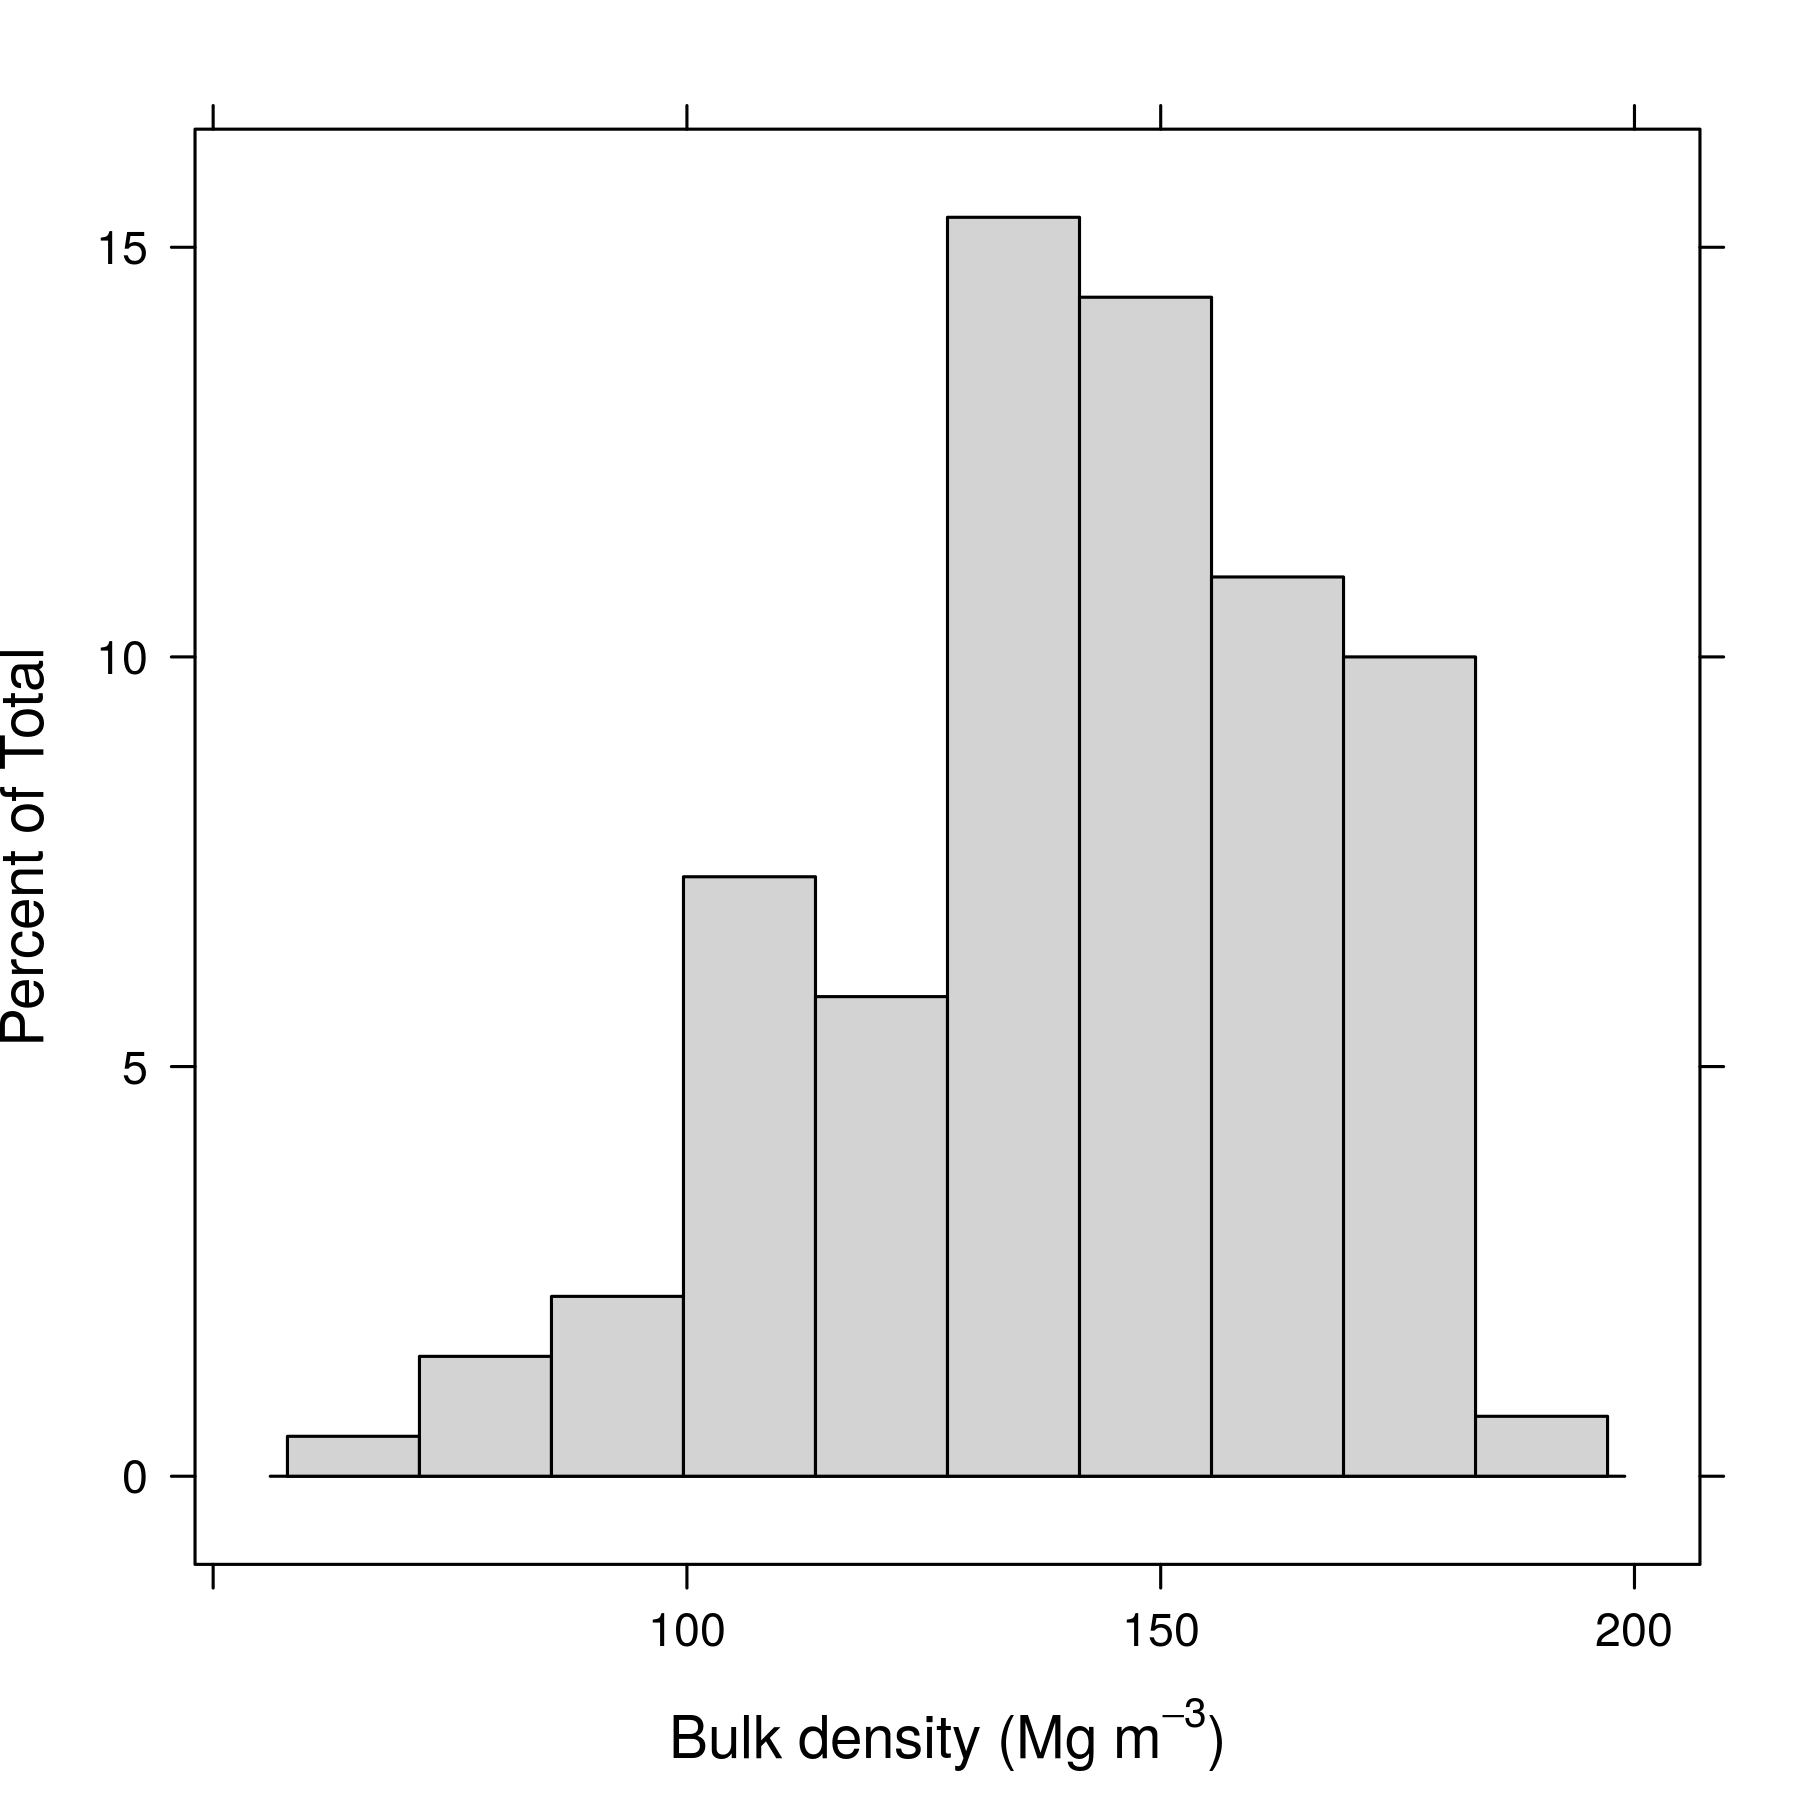
\includegraphics[width=0.60\textwidth]{fig/chap04-bude}
\caption[Distribution of bulk density in the Santa Maria dataset.]{Distribution of bulk density 
(\si{\mega\gram\per\cubic\metre}) in the Santa Maria dataset.}
\label{fig:chap04-bude}
\end{figure}

The bulk soil density was not determined in the locations where the soil was very shallow or stony.

\subsection{Exchangeable Bases and Acidity}
\label{chap:chap04-ecec}

The exchangeable calcium (\texttt{CALC}, \si{\milli\mole\per\kilo\gram}) and magnesium (\texttt{MAGN}, 
\si{\milli\mole\per\kilo\gram}) were determined by atomic absorption spectroscopy after extraction with 
\SI{1.0}{\mole\per\liter} \ce{KCl} solution \cite{ClaessenEtAl1997}. The exchangeable sodium (\texttt{SODI}, 
\si{\milli\mole\per\kilo\gram}) and potassium (\texttt{POTA}, \si{\milli\mole\per\kilo\gram}) were extracted 
with a \SI{0.05}{\mole\per\liter} \ce{HCl} solution plus \SI{0.025}{\mole\per\liter} \ce{H2SO} 
(Mehlich-\num{1} solution). Both were quantified by means of flame atomic emission spectrometry 
\cite{TedescoEtAl1995}.

The exchangeable acidity (\texttt{EXAC}, \si{\milli\mole\per\kilo\gram}) was extracted using the same 
\SI{1.0}{\mole\per\liter} \ce{KCl} solution used to extract the exchangeable calcium and magnesium. It was 
determined by titrimetry with \SI{0.025}{\mole\per\liter} \ce{NaOH} solution \cite{ClaessenEtAl1997}.

% TODO: Include POAC in the database and improve the description of how it was determined.
% The potential acidity (POAC, \si{\milli\mole\per\kilo\gram}) was determined with \SI{1.0}{\mole\per\liter} 
% calcium acetate solution at pH~\num{7.0} and titrated with \SI{0.0606}{\mole\per\liter} \ce{NaOH} solution 
% as described by \citeonline{ClaessenEtAl1997}.

\begin{figure}[!ht]
\centering
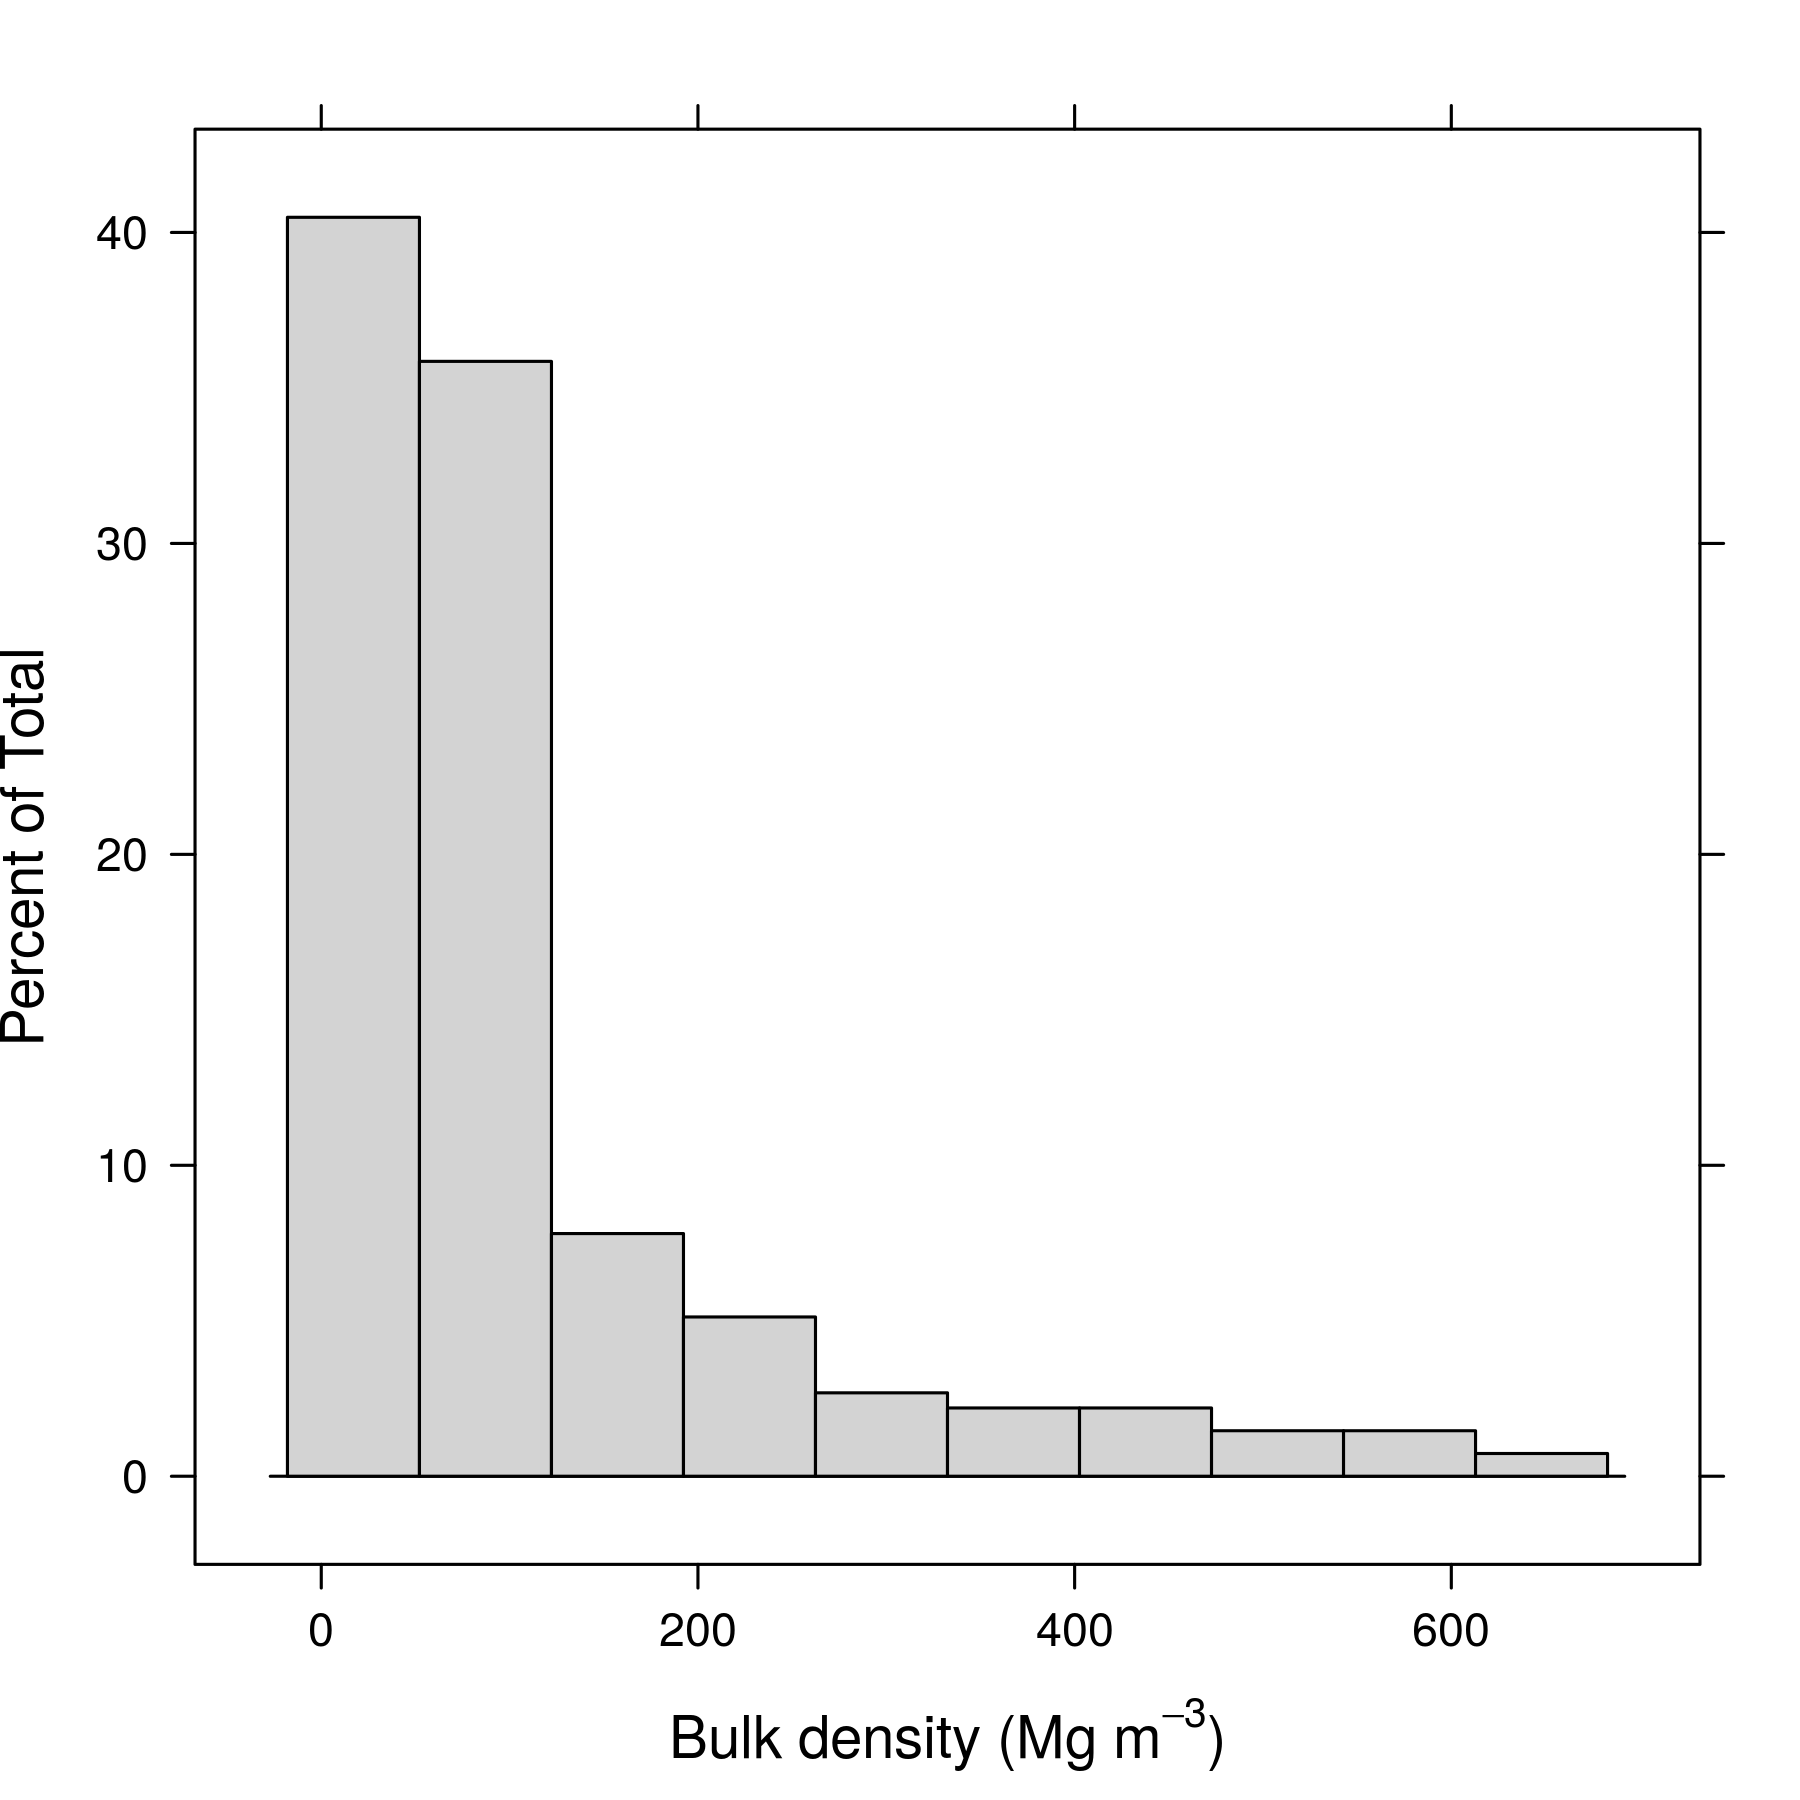
\includegraphics[width=0.60\textwidth]{fig/chap04-ecec}
\caption[Distribution of effective cation exchange capacity in the Santa Maria dataset.]{Distribution of 
effective cation exchange capacity (\si{\milli\mole\per\kilo\gram}) in the Santa Maria dataset.}
\label{fig:chap04-ecec}
\end{figure}

The effective cation exchange capacity (ECEC, \si{\milli\mole\per\kilo\gram}) was defined as the sum of 
exchangeable bases and exchangeable acidity (\autoref{fig:chap04-ecec}), i.e. 

\begin{equation*}
 \texttt{ECEC} = \texttt{CALC} + \texttt{MAGN} + \texttt{POTA} + \texttt{SODI} + \texttt{EXAC}.
\end{equation*}

% TODO: Provide a more detailed description of how these are calculated and include the data in the database.
% The sum of exchangeable bases (BASES) is given by the sum of the exchangeable calcium, magnesium, sodium and 
% potassium. The effective cation exchange capacity (ECEC) is given by the exchangeable acidity plus the 
% sum of exchangeable bases. The potential cation exchange capacity (CEC) is given by the potential acidity 
% plus the sum of exchangeable bases. Note that the standard method for determining exchangeable bases relies 
% on the use of barium chloride [BaCl$_2$]. The base saturation (BASA) is given by the sum of exchangeable 
% bases divided by the potential cation exchange capacity. The saturation of the ECEC with exchangeable 
% acidity, or the aluminum saturation (ALSA), is given by the sum of exchangeable bases divided by the 
% effective cation exchange capacity. The results are multiplied by 100. 

% \begin{figure}[!ht]
% \centering
% <<echo = FALSE>>=
% options(useFancyQuotes = FALSE)
% tmp <- read.table(
%  '~/projects/dnos-sm-rs/dnos-sm-rs-general/data/labData.csv', sep = ";",
%  header = TRUE, na.strings = 'na')
% lattice::trellis.par.set(
%  fontsize = list(text = 16, points = 15), axis.line = list(lwd = 0.01),
%  layout.widths = list(left.padding = 0, right.padding = 0),
%  layout.heights = list(top.padding = 0, bottom.padding = 0))
% aa <- pedometrics::plotHD(tmp$CLAY, xlab = 'CLAY')
% bb <- pedometrics::plotHD(tmp$ORCA, xlab = 'ORCA')
% cc <- pedometrics::plotHD(tmp$ECEC, xlab = 'ECEC')
% dd <- pedometrics::plotHD(na.exclude(tmp$BUDE), xlab = "BUDE")
% @
% \begin{minipage}[b]{63mm}
% \subcaption{}
% \centering
% <<intro-clay, fig = TRUE, echo = FALSE>>=
% print(aa)
% @
% \end{minipage}
% \begin{minipage}[b]{63mm}
% \subcaption{}
% \centering
% <<intro-orca, fig = TRUE, echo = FALSE>>=
% print(bb)
% @
% \end{minipage}
% \begin{minipage}[b]{63mm}
% \subcaption{}
% \centering
% <<intro-ecec, fig = TRUE, echo = FALSE>>=
% print(cc)
% @
% \end{minipage}
% \begin{minipage}[b]{63mm}
% \subcaption{}
% \centering
% <<intro-bude, fig = TRUE, echo = FALSE>>=
% print(dd)
% @
% \end{minipage}
% \caption{The four soil properties explored in this thesis: (a) clay content, (b) organic carbon
% content, (c) effective cation exchange capacity, and (d) bulk density. Each panel shows the sample
% histogram and summary statistics of the soil properties in their original scale ($\lambda = 1$), as
% well as the theoretical probability density function so that we can assess how good is the fit of
% the normal distribution to the data -- a product of the \Rpackage{pedometrics}.}
% \label{fig:intro-soil-properties}
% \end{figure}

% \section{CONCLUSIONS}
% 
% The main goal of documenting the soil data contained in the Santa Maria dataset was to provide the reader 
% the basis to understand the soil data used in the thesis, and also to support future soil spatial modelling 
% exercises in the catchment of the DNOS reservoir.
% 
% As a result of an ongoing collaborative effort, this documentation will be improved in the near future as 
% new studies are developed. We plan to include new figures to exemplify how field soil sampling was carried 
% out. Details of non-standard soil description and analysis methods will likely be extended. This includes 
% the oxidative treatment with \ce{H2O2} to which soil samples were submitted prior to particle size 
% distribution analysis. For cases such as the ECEC, determined using a non-standard method, we plan to 
% develop a study to calibrate a model to convert our results to the standard method for determining 
% exchangeable bases, which uses barium chloride (\ce{BaCl2}) for saturation.
% 
% Other already existing soil data will also be included in the Santa Maria dataset and documented as well. 
% These data have not been used in any study so far, including the potential acidity, sum of exchangeable 
% bases, potential cation exchange capacity, base saturation, aluminium saturation, and the five size classes 
% of the sand fraction.
% 
% Once a comprehensive documentation of the existing soil data has been constructed, we will prepare a basic 
% spatial exploratory soil data analysis. We hope that our effort to properly document the soil data that we 
% produced, and make it freely available for use, will serve as an example for future soil spatial modelling 
% studies developed elsewhere.
